\chapter{Introduction}
\label{chap:intro}
\minitoc


 \section{Le domaine du Calcul Haute Performance} 
 

%---------------------------------------------------------------------------------

Le domaine du \gls{hpc} n'est pas apparu de lui même, c'est un moyen qui à été crée par les scientifiques et plus particulièrement ceux travaillant dans la simulation numérique. La simulation numérique est le procédé qui permet de simuler un phénomène physique sur un ordinateur par la programmation. Elle a de nombreux avantages comme celui de pouvoir simuler des phénomènes dont les conditions ne sont pas reproductibles sur terre comme dans le  domaine de la physique appliquée. Elle élargie donc les domaines explorables ce qui rend son champs d'application presque infini.  


 \subsection{Le calcul scientifique et la simulation numérique}


Les simulations sont aujourd'hui un pilier stratégique de nombreuses entreprises qui travaillent dans des domaines très différents. Pour mieux comprendre les changements qu'elle a apportée à l'industrie prenons l'exemple de l'industrie automobile et du crash de voiture. Les tests de crash de voitures ne sont plus réalisés avec de vraies voitures, les voitures sont simulées sur ordinateurs et envoyées percuter des murs virtuels. Cette technique à un impact conséquent sur le travail des ingénieurs. Elle a pour effet de réduire les temps de conception, car il n'y plus besoin de créer une voiture avec les matériaux à tester. On peut dans la même journée créer un modèle avec un matériau, lancer la simulation le temps du repas, analyser les résultats et relancer une simulation dans la nuit. Le gain de temps est énorme comparé à si on devait construire la voiture de toute pièce pour ensuite la tester sur un vrai mur. Le second gain, qui est fortement lié au premier, est la réduction des coûts de conceptions, plus besoin de faire construire des nouveaux matériaux pour se rendre compte au bout d'un essai qu'ils ne correspondent pas au besoin du constructeur. 



 
Les domaines qui ont recours au \gls{hpc} sont nombreux notamment à travers la simulation numérique qui devient un levier d'action essentiel pour beaucoup d'industries. Pour la compétitivité et l'innovation des entreprises, les simulations numériques sont désormais un outil indispensable d'aide à la conception, à la décision et au contrôle de leurs activités. Le schéma \ref{fig:tikz_simulation} montre comment la simulation numérique est venue révolutionner de nombreux domaines scientifiques.


%TikZ picture
\begin{figure}
\begin{center}

\begin{minipage}[]{.5\textwidth}

\begin{tikzpicture}[->,shorten >=1pt,auto,node distance=3.8cm,   scale=0.49, every node/.style={transform shape}]
  \tikzstyle{every state}=[fill=none,draw=black,text=black,  , font=\bf]
  \tikzstyle{edge_style} = [draw=black, line width=2, ultra thick]
  \tikzstyle{node_style} = [circle,draw=blue,fill=blue!20!,font=\sffamily\Large\bfseries]


  \node[state]					    (A)                     {Nature};
  \node[state]        				(B) [below of=A]        {Observations};
  \node[state,]         		    (D) [below right of=B]  {Théorie};
  \node[state, align=left]         	(C) [below left of=B]   {Expérience\\ physique};

  \path
		(A) edge [edge_style]   node {} (B)
        (B) edge [edge_style]   node {} (D)
        (C) edge [edge_style]   node {} (B)
        (D) edge [edge_style]   node {} (C);
\end{tikzpicture}
\end{minipage}%
\begin{minipage}[]{.5\textwidth}

\begin{tikzpicture}[->,shorten >=1pt,auto,node distance=3.8cm,   scale=0.49, every node/.style={transform shape}]
  \tikzstyle{every state}=[fill=none,draw=black,text=black,  , font=\bf]
\tikzstyle{edge_style} = [draw=black, line width=2, ultra thick]
\tikzstyle{node_style} = [circle,draw=blue,fill=blue!20!,font=\sffamily\Large\bfseries]


  \node[state]					(A)                    {Nature};
  \node[state]        					(B) [below of=A] {Observations};
  \node[state,]         					(D) [below right of=B] {Théorie};
  \node[state, align=left]         	(C) [below left of=B] {Expérience\\ physique};
  \node[state, align=left]        	(E) [left of=C]       {Simulation\\numérique};

  \path
		(A) edge [edge_style]            node {} (B)
        (B) edge [edge_style]     node {} (D)
        (C) edge [edge_style]           node {} (B)
        (D) edge [edge_style]             node {} (C)
              edge [edge_style, bend left]     node {} (E)
        (E) edge [edge_style, bend left]  node {} (B);
\end{tikzpicture}


\end{minipage}
\end{center}


 \caption{La simulation numérique a apportée une nouvelle façon d'expérimenter les théories \cite{BSC_FIB_SCA}} 
 \label{fig:tikz_simulation}
 \end{figure}

A l'origine, les scientifiques observaient la nature et émettaient des théories pour expliquer ces observations. En se basant sur ces théories ils réalisaient des expériences physiques pour les valider ou non. Il faisaient alors de nouvelles observations pour affiner leur théorie. Les simulations numériques sont alors apparues comme des alternatives aux expériences physiques qui étaient souvent longues et onéreuses. Avec l'apparition d'ordinateurs de plus en plus puissant on pouvait donc les programmer pour simuler des expériences sans avoir à les réaliser. Les gains de temps et d'argent étant alors conséquents.

La simulation numérique est un domaine ou les programmes sont utilisés pour simuler un phénomène réel (physique, chimique, biologique, etc.). Cette approche est largement utilisée en science pour prédire l'évolution d'un phénomène dans le temps et l'espace. La majorité de ces simulations son basés sur des équations dites \textit{gouvernantes} qui sont des approximations des phénomènes étudiés. Comme les ordinateurs ne peuvent pas exécuter une infinité d'instructions, ces équations ne peuvent pas être utilisées directement et ont besoin d'être discrétisé. En mathématiques, la discrétisassions est un procédé  qui permet de passer d'une fonction, d'un modèle ou d'une équation continue à son équivalent continu (\autoref{pic_maillage}). Ce procédé ne permet pas de décrire le phénomène réel, mais de l'approximer avec plus ou moins d'erreur. Pour améliorer ces simulations, ces représentations doivent utiliser des maillages le plus fin possible. C'est en cela que ces simulations nécessitent d'énormes puissances de calculs et que cette demande est illimité car les maillages pourront toujours être affinés. 

\begin{figure}
    \center
    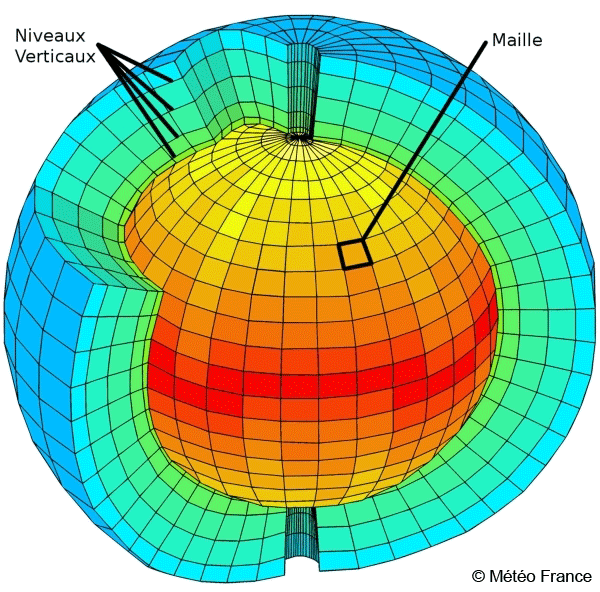
\includegraphics[width=4cm]{images/Chapitre1/maillage.png}
    \caption{\label{pic_maillage} Le maillage le plus fin exploité par Météo-France pour ses prévisions régionales restitue des mailles de 2,5 km de côté. (source \url{www.irma-grenoble.com})}
\end{figure}




\begin{enumerate}
\item Aéronautique: la Dynamique des Fluides (CFD) est utilisée pour valider qu'un flux d'air circule correctement autour des ailes pour essayer de maximiser le portage des ailes. 
\item Industries des hydrocarbures: la recherche pétrolière utilise le HPC pour analyser les fonds marins et modéliser les réservoirs de pétrole pour optimiser leur extraction.
\item Météorologie: pour améliorer les prédictions météorologiques mais aussi de les réaliser plus longtemps à l'avance. 
\item Sciences biologique: séquençage et alignement ADN, découverte de drogues 
\end{enumerate}



%%%%%%%%%%%%%%%%%%%%%%%%%%%%%%%%%%%%%%%%%%%%%%%%%%%%%%%%%%%%%%%
%%%%%%%%%%%%%%%%%%%%%%%%%%%%%%%%%%%%%%%%%%%%%%%%%%%%%%%%%%%%%%%
%%%%%%%%%%%%%%%%%%%%%%%%%%%%%%%%%%%%%%%%%%%%%%%%%%%%%%%%%%%%%%%
%%%%%%%%%%%%%%%%%%%%%%%%%%%%%%%%%%%%%%%%%%%%%%%%%%%%%%%%%%%%%%%

\subsection{Définition du Calcul Haute Performance}
 
 Le domaine du HPC est le domaine informatique qui consiste à regrouper des puissances de calculs pour qu'ensemble elles travaillent à la résolution d'un problème partagé. Comme expliqué dans la section précédente, la simulation numérique est utilisée dans des domaines très différents. Le point commun de ces applications est la résolution d'un gros problème qui ne peut pas être résolu par une seule ressource. Ce problème est divisé en sous-problème de petites tailles, qui eux peuvent être résolus séparément. Cette méthode de résolution est appelée le calcul parallèle, un exemple est donné dans la partie \ref{sub_reso_partage}. Aujourd'hui, les utilisateurs de HPC peuvent accéder à ces clusters par différents moyens:
\begin{enumerate}
\item \textbf{Dedicated supercomputer}, une architecture unique est créée. La conception de ces architectures étant unique, les frais de conception sont très élevés mais cette spécificité en fait des architectures très performantes car elles sont conçues spécialement pour répondre à un besoin précis. 
\item \textbf{Le Commodity cluster}, qui agrège du matériel grand public (haut de gamme) pour former des grappes de calculs de plusieurs milliers de processeurs.
\item \textbf{HPC as a service} ou HPC Cloud ou encore HPC dans le nuage,  utilise le modèle \textit{System as a Service} pour apporter aux entreprises manquant de moyens ou de compétences un accès à une infrastructure HPC externalisée. L'un des principaux avantages est la flexibilité d'usage (adapter l'infrastructure à son besoin). 
\item \textbf{Grid Computing} ou grille informatique est un regroupement de ressources informatique à grande échelle (nationale voir internationale). Par exemple \textit{Einstein@Home} \cite{PhysRevD.80.042003} est un projet de recherche mondial sur les ondes gravitationnelles  qui regroupe les ordinateurs de 50000 utilisateurs connectés à travers le monde qui sont utilisés pour  analyser les données transcrite par des capteurs.
\end{enumerate}


Quel que soit le moyen de conception et d'utilisation, ces architectures sont des regroupements de centaines, voire de milliers de ressources qui forment une grappe de serveur que l'on appelle un \textit{cluster} ou \textit{supercalculateur}. 

\subsubsection{Le marché du HPC}
Il y a plusieurs catégories d'acheteurs de cluster HPC qui n'ont pas tous les mêmes besoins et les mêmes budgets:
\begin{itemize}
    \item Le petit HPC: ce sont les clients avec les plus petits budgets comme par exemple des équipes d'ingénieurs ou des petites universités qui ont besoin d'un cluster de calcul pour des usages personnels. On pourra citer le projet SIMSEO qui à pour but de sensibiliser et d'accompagner les PME à utiliser la simulation numérique. Car même pour des entreprises de tailles réduite, la simulation et le HPC peuvent être des atouts clefs dans leur stratégie.
    \item Le HPC public: il regroupe les grandes universités qui partagent le matériel entre plusieurs écoles ou laboratoires de recherche. Ces systèmes sont d'une puissance élevée, et certains sont classé dans le \textit{TOP500}. Les codes exécutés sont souvent disponibles en open-source.
    \item Le HPC commercial: ce sont tous les clusters que les entreprises privées utilisent pour développer leur business. Les applications qui y sont exécutées sont souvent des applications privées.
\end{itemize}



%%%%%%%%%%%%%%%%%%%%%%%%%%%%%%%%%%%%%%%%%%%%%%%%%%%%%%%%%%%%%%%
%%%%%%%%%%%%%%%%%%%%%%%%%%%%%%%%%%%%%%%%%%%%%%%%%%%%%%%%%%%%%%%
%%%%%%%%%%%%%%%%%%%%%%%%%%%%%%%%%%%%%%%%%%%%%%%%%%%%%%%%%%%%%%%
%%%%%%%%%%%%%%%%%%%%%%%%%%%%%%%%%%%%%%%%%%%%%%%%%%%%%%%%%%%%%%%

\subsection{Les Clusters}
\begin{fancyquotes}
Un cluster (grappe) de serveurs est un \textbf{interconnexion} de \textbf{ressources informatiques} dans le but de \textbf{résoudre un problème} complexe de façon \textbf{partagée}. 
\end{fancyquotes}

A l'origine les premiers supercalculateurs étaient des architectures uniques crées de toutes pièces pour un client. Il était alors très dure de les reproduire ensuite rendant leur coût de conception très élevé. Seymour Cray présenta le premier super- calculateur en 1960 alors qu'il travaillait pour Control Data Corporation. A partir des années 1990 apparurent des clusters construits à partir de matériels haut de gamme mais qui peuvent s'acheter dans la grande distribution. Ce n'est donc pas la puissance individuelle de ces matériels qui est importe mais c'est le regroupement de centaines de stations de travail qui en fait des supercalculateur, et cette façon de les construire est toujours la même aujourd'hui.\\



%%%%%%%%%%%%%%%%%%%%%%%%%%%%%%%%%%%%%%%%%%%%%%%%%%%%%%%%%%%%%%%
%%%%%%%%%%%%%%%%%%%%%%%%%%%%%%%%%%%%%%%%%%%%%%%%%%%%%%%%%%%%%%%

\subsubsection{L'interconnexion } 
La liaison des serveurs se fait grâce au meilleurs technologies de réseaux pour atteindre le maximum de performances. Les caractéristiques principales de ces réseaux sont une latence faible et une bande passante élevée. Le terme de \textit{latence} fait référence au temps qu'il faut à un message (ou paquet de bits) pour aller d'un serveur à un autre. On utilise alors la milliseconde ou nano seconde comme unité. La bande passante quand à elle représente le nombre de messages qui peuvent être transporté en même temps entre deux serveurs, on utilise l'unité du gigaoctet. En simplifiant beaucoup; on peut voir le réseaux comme un tuyau, la vitesse de l'eau y circulant étant la latence, et son diamètre la bande passante. Et suivant le type d'application, la priorité n'est pas la même. On peut citer le domaine de la finance qui à besoin d'un réseaux extrêmement rapide pour exécuter des milliers d'opérations à la seconde. Alors qu'un hébergeur vidéo sera très sensible à la bande passante de son système pour pouvoir fournir du contenus à plusieurs clients.
Aussi, l'efficacité du réseau ne dépend pas seulement du matériel, la partie logiciel est tout aussi importante: des algorithmes de routages à la complexité des protocoles, tout est importants pour faciliter la livraisons des paquets de données. Enfin, la structures des switchs doit être bien pensée pour réduire le nombre de \textit{sauts} de chaque échanges, c'est à dire le nombre d'intermédiaire pour aller de l'expéditeur au destinataire. La figure \ref{pic_topologie} montre un exemple de topologie et l'impact qu'elle a sur la latence des communications qui peut être multiplié par deux suivant à qui la machine A s'adresse. Cette structure (ou topologie) doit s'assurer d'éviter tout risques de congestions afin qu'une partie de réseau ne soit pas trop sollicitée ce qui créerait des baisses de performances. 

\begin{figure}
    \center
    \includegraphics[width=4cm]{images/Chapitre1/TopologieReseau.png}
    \caption{\label{pic_topologie} Exemple d'une topologie d'un cluster. Si le serveur A veut envoyer un message à B, il devra effectuer 4 sauts (ou \textit{hop}).}
\end{figure}


%%%%%%%%%%%%%%%%%%%%%%%%%%%%%%%%%%%%%%%%%%%%%%%%%%%%%%%%%%%%%%%
%%%%%%%%%%%%%%%%%%%%%%%%%%%%%%%%%%%%%%%%%%%%%%%%%%%%%%%%%%%%%%%

\subsubsection{Les ressources informatiques} 
Les serveurs de calculs connectés grâce à ces réseaux ont aujourd'hui beaucoup de points communs et dépendent de moins en moins du vendeur qui les a conçus. Un cluster moderne est construit avec du \textit{commodity hardware}, du matériel produit en série. Que ce soit des processeurs à la mémoire, on peut trouver ces matériels sur le marché grand public. C'est seulement l'agglomération de ces serveurs par centaines, qui en fait des architectures unique et très puissante. Aujourd'hui la majorité des architectures systèmes est composée d'un serveur contenant un ou plusieurs processeurs qui est relié à sa mémoire, son disque et qui peut être accompagné d'accélérateurs comme des carte graphiques. Même si la majorité des architectures se ressemble cela ne les rend pas pour autant moins complexes car chaque composants cités précédemment est d'une complexité sans fin. Les mémoires par exemple compte des dizaines de technologies différentes avec chacune leur avantages et leurs inconvénients. De même que pour les processeurs qui sont au fil des années se sont complexifiés pour répondre à des besoins particuliers. L'élaboration d'un cluster doit donc prendre en compte tout ces aspects mais aussi les contraintes inhérente au projet (le prix, l'espace disponible ou la puissance électrique disponible). 

% ---------
\subsubsection{Résolution partagée}
L'interconnexion de toutes ces ressources est réalisée dans le seul but de réduire le temps nécessaire à la résolution d'un problème. En effet, pour une expérience donnée si l'on possède un cluster de 1000 machines on ne voudra pas réaliser l'expérience un millier de fois mais plutôt réduire le temps d'une expérience par un facteur 1000 pour ensuite analyser les résultats, changer les paramètres et pouvoir lancer une nouvelle expérimentation. La calcul parallèle est un ensemble de moyens, logiciel et matériel qui permettent de réaliser des instructions simultanément. L'idée principale du calcul parallèle est de réduire le temps de calcul d'un programme en divisant le travail à réaliser, le partager en sous-problèmes qui peuvent être résolu de façon indépendante par plusieurs ressources de calcul, comme des processeurs. Un exemple concret de résolution d'un problème grâce à la programmation parallèle est donnée dans la section \ref{sub_reso_partage}
\textbf{TODO fini cette section, une image}


% ---------


\subsubsection{Le TOP500 et le benchmark HPL}

\paragraph{Le benchmarking ou l'étalonnage} est une pratique courante qui consiste à évaluer plusieurs solutions en leur faisant passer un épreuve commune. Dans le domaine informatique cela permet de tester différentes architectures matériels et d'évaluer laquelle sera la plus performantes. Il existe plusieurs benchmark qui ont chacune leur particularités. Ces codes essayent de reproduire les opérations faites par des codes industriels, dans le but de faire des projections de performances et pouvoir comparer deux solutions. Le benchmark le plus populaire dans le domaine du HPC est celui développé par Jack Dongara en 1988: le benchmark HPL \cite{Dongarra}. C'est grâce à lui que le classement du TOP500 est réalisé deux fois par ans.


\paragraph{Le TOP500} \footnote{\url{www.top500.org}} est un classement mondial qui classe, tous les 6 mois depuis 1993, les 500 super-calculateurs les plus puissants au monde. Ce classement se base sur le nombre maximum d'opérations flottantes qui peuvent être exécutées en une secondes. Cette unité à été choisie car la grande majorité des codes utilisés dans les domaines précédemment cités, exécutent des opérations sur des nombres flottant. Il s'avère donc judicieux de choisir ce dénominateur commun pour comparer les différentes architectures.  Une opération flottante peut être traduite par \textit{floating point operation} ou FLOP en anglais, on parlera donc de FLOP/S ou FLOPS pour désigner le nombre d'opérations flottante par seconde. Pour réaliser ce benchmark tous les supercalculteurs doivent exécuter le même code, le benchmark LINPACK \cite{Dongarra} \cite{450b1baca0774fd0976ff739b90bed04}. Ce benchmark est un code simple qui résout un système d'équation linéaire de deux matrices $A$ et $B$ par $Ax = B$. L'avantage de ce code est que les performances évoluent linéairement avec le nombre de machines utilisées car il y a très peu de communication sur le réseaux. Le résultat est un nombre de FLOP/S que la machine peut exécuter, ce qui rend la comparaison avec d'autres supercalculateur facile. 



Le site web du \textit{top500} contient de nombreuses données. On peut par exemple voir la consommation électrique, le nombre de coeurs, ou encore si les clusters contiennent des cartes graphique. Sur le graphique \ref{pic_top500perf_evo}, on voit que la puissances des supercalculateurs augmente d'un facteur 1000 tous les 10 ans.
Il faut cependant savoir que ce classement ne contient pas toutes les machines. En effet, certains industriels ne préfèrent pas paraître dans ce classement. Stratégiquement parlant, il peut être intéressant de ne pas publier sa puissance de calcul et nous savons que les clusters les plus puissants n'y figurent pas. Cependant ce classement nous permet de voir les tendances que suivent la majorité des architectures pour comprendre comment elles évoluent.\\

\begin{figure}
    \center
    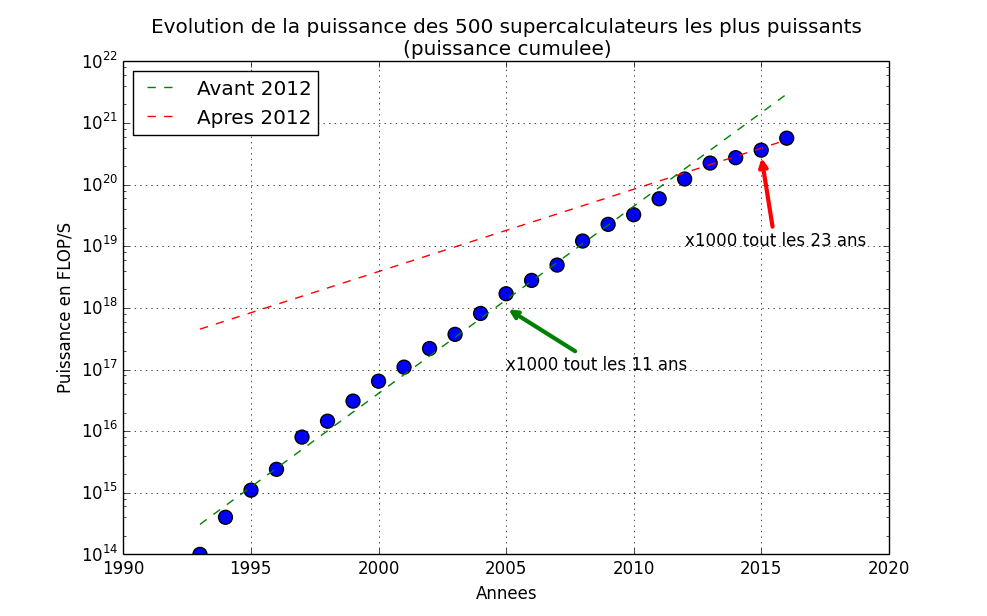
\includegraphics[width=10cm]{images/Chapitre1/pic_top500perf_evo.png}
    \caption{\label{pic_top500perf_evo} Évolution de la performance cumulée des 500 supercalculateurs les plus puissants au monde. La pente de l'évolution diminue à partir de 2012}
\end{figure}


Il existe un second classement qui classe les supercalculateur en fonction de leur ratio $\frac{FLOPS}{WATT}$ nommé le \textit{Green500} \cite{feng2007green500}. Comme nous allons le voir ensuite, la consommation électrique est devenus une contrainte forte dans l'architecture des nouveaux cluster. De plus en plus, la question n'est plus de construire le supercalculateur le plus puissant, mais le plus efficace.

\subsubsection{HPC ou HTC}
Aujourd'hui le domaine des supercalculateurs est souvent désigné par le terme HPC, mais il y a quelques précision à apporter quant à la mauvaise utilisation de ce terme. Il existe un autre domaine qui utilise les supercalculateur, le High Throughput Computing (HTC). En effet, la communauté à voulu donner un nom aux architectures capables d'exécuter différentes applications simultanément et ce sans interruptions sur plusieurs mois. Contrairement aux applications HPC qui exécutent des taches très dépendantes les unes des autres, les applications HTC se focalisent sur l'exécution des plusieurs tâches en parallèles et assure la disponibilité maximale du nombre de ressources dont dispose le supercalculateur. Prenons pour exemple un cluster de calcul partagé dans une université. L'objectif de cette machine n'est pas d'exécuter une application toute l'année, mais plutôt de répartir le matériel disponible entre les utilisateurs pour que tous puissent l'utiliser au maximum. Une majorité des clusters d'aujourd'hui fonctionnent sur le même modèle et l'utilisation de l'expression HPC pour les désigner est en fait un abus de langage.



% ------------------------------------



\section{Le domaine du HPC en 2017: challenges et contraintes}


\begin{fancyquotes}
Peu importe quelle puissance attendront les processeurs, le logiciel trouvera toujours une façon d'utiliser cette puissance. Construisez un processeur 10 fois plus rapide, et la partie logiciel trouvera toujours 10 fois plus à faire (ou le fera 10 fois moins efficacement)  \cite{sutter2005software}
\end{fancyquotes}


Dans cette section nous allons tout d'abord exposer quels sont les challenges du HPC en 2017, pourquoi nous en avons besoin plus que jamais. Dans une seconde partie nous aborderons les contraintes qui empêchent les super-calculateurs de continuer à augmenter leur puissance d'années en années comme cela se faisait jusqu'à maintenant.

\subsection{Les challenges et opportunités}

La création de cette collaboration entre l'école de l'ENS et HPE n'est pas due au hasard. Cette thèse a été créée alors que le domaine du HPC connais un ralentissement sans précèdent (graphique \ref{pic_top500perf_evo}. Depuis 2012 certaines barrières ont été atteintes et les processus qui permettaient aux architectures d'évoluer à cadence constante ne sont plus viables. 




\subsubsection{Exascale}
Aujourd'hui nous rencontrons des utilisations du HPC tous les jours, que ce soit quand nous regardons la télévision ou que nous consultons le cours de la bourse. Le HPC à un réel impacte sur nos vie, les rendant plus sécurisées en prévoyant précisément des catastrophes naturelles. tous les jours de nouvelles applications sont découvertes, et certaines ne sont techniquement pas envisagées car elles nécessiteraient trop de puissances de calculs. L'objectif de tous les constructeurs présent dans le domaine du HPC est la construction du premier ordinateur capable de réaliser  $10^18$ opérations sur des nombres rationnels par secondes, l'équivalent d'un \textit{exaflop} ($10^18$ Floating Point Operations). L'industrie s'est donc lancée dans cette course effrénée à l'exaflop. En effet, le premier constructeur qui y parviendra bénéficiera d'un grand coup marketing et acquerra de nombreux clients car la majorité des clients ont des problèmes ne pouvant être réglé que par un ordinateur de cette puissance, et attendent son arrivé.

\subsubsection{De nouveaux clients}
L'arrivée de l'exaflop va entrainer l'arrivée de nouveaux clients, et il est indispensable pour des constructeurs comme HPE d'être prêt à les accompagner. Avec l'apparition des objets connectés le monde connaît une explosion des données qui sont générées et collectées. Elles sont ensuite stockées dans des data centers, qui n'ont pas les puissances suffisantes pour pouvoir les analyser. En effet les données générées par les montres, les frigos connectés ou les capteurs dans des chaînes de productions n'ont pas réelle utilité si elles ne sont pas exploité grâce à des techniques de \textit{Data Mining}. Et l'arrivée du machine learning nous ouvre à un monde extraordinaire qui n'est possible que si nous créons les architectures adéquats pour en profiter. Un autre domaine nécessitant ces quantités de calculs est celui de la recherche médicale et biologique. Aujourd'hui nous sommes capables de simuler des réactions chimiques de quelques nano secondes et sur de petit volumes. La création de supercalculateur exaflopique serait une énorme avancée pour ces clients, et les constructeurs qui n'auront pas misé sur l'exascale seront terriblement impactés. Ces nouveaux clients sont une grosse opportunité pour une entreprise comme HPE. Une analyse de marché paru en 2016 montre que le marché du High Performance Computing pèsera 36 milliards de dollars en 2020, alors qu'il en valait 28 en 2015\footnote{\url{http://www.marketsandmarkets.com/Market-Reports/Quantum-High-Performance-Computing-Market-631.html}}. Cette augmentation de 5\% par année est due à l'explosion des quantités, à la complexité des techniques pour les analyser et les visualiser et de la demande grandissante de solution HPC dans de nombreux domaines.


\subsubsection{Les nouvelles technologies}
Dans l'objectif de construire des supercalculateur toujours plus puissant nous pouvons et allons pouvoir nous appuyer sur des évolutions technologiques majeures. En effet que ce soit au niveau des mémoires avec l'arrivée des mémoire non-volatile (NVM memory), ou au niveau des réseaux avec la photonics. Il va falloir que, constructeur comme client, se tienne à jour de toutes ces évolutions technologique qui vont modifier les façon de programmer et de construire les architectures. HPE à un un projet de machine exascale nommé The Machine. Cette architecture très novatrice s'appuie sur trois piliers technologiques: les mémoires \textit{memristors} et les réseaux à base de fibre: la \textit{ photonic}. La troisième avancée et la restructuration complète de l'architecture d'un super calculateur grâce au protocole de communication Gen-Z.\\

%*****************************************************************************************************

\subsection{Les contraintes}
La loi de Moore prevoyait une augmentation exponetielle de la puissance des processeurs, mais une telle augmentation ne peut pas continuer indéfiniment car nous avons atteints certaines limites physiques. La course à l'exascale est lancée mais il existe beaucoup de contraintes qui ralentissent et compliquent ce challenge technologiques. Les contraintes sont multiples et n'influe pas autant sur les performances, mais depuis 2012 on assiste à un changement de dynamique (voir le graphique \ref{pic_top500perf_evo}). Cette partie liste donc les contraintes majeures qui impactent le domaine du calcul haute performance.


\subsubsection{Électrique}
L'électricité est une forte contrainte dans l'élaboration de ces clusters et elle est un facteur majeur du ralentissement de l'évolution des performances des super-calculateur du TOP500 vu sur la figure \ref{pic_top500perf_evo}. En effet, aujourd'hui les puissances électriques nécessaires pour alimenter ces machines dépasse la capacité des lignes électriques qui arrivent jusqu'aux centre de calculs. Notre stratégie d'augmenter le nombre de serveurs pour augmenter la puissance totale n'est plus valable. Ce problème n'est pas nouveau et de nombreux efforts ont déjà était fait sur les alimentations et le refroidissement qui sont proche de l'idéal. Nous avons tendance à penser que l'investissement dans un super-calculateur est réaliser lors de son achat, mais un budget conséquent doit être alloué pour son alimentation. En simplifiant, on peut ramener le prix de l'électricité à 1 dollar par watt durant une année. Si on regarde la consommation électrique des clusters du Top500, on constate qu'en moyenne ils consomment 1.4 mégawatt et que les 5 qui consomment le plus sont au dela de 12 mégawatt (voir graphique \ref{pic_top500_power}). Facilement on calcul que l'alimentation de ces architectures coûte des millions de dollars chaque années (20 millions de dollars pour le premier).
L'objectif est donc d'augmenter le nombre de calcul que l'on réalise pour une puissance électrique donnée, c'est à dire augmenter le ratio $\frac{FLOP}{Watt}$. PathForward à récemment publié les exigences technique auxquelles supercalculateur exascale allé devoir répondre \cite{PathForward_Req}. Cette étude montre qu'un système exascale ne devra consommer entre 20 et 30 megawatt. Ce qui n'est pas si loin de la consommation des deux clusters les plus puissant (19 et 18 mégawatt). D'autant plus si on compare au saut de performances que l'on doit faire pour atteindre l'exaflop. Il va falloir avec 50\% d'énergie en plus, réaliser 30 fois plus d'opérations. L'écart entre ces deux facteurs va nous obliger à repenser à comment les codes sont exécutés et dans un second temps de repenser entièrement les architectures.


\begin{figure}
    \center
    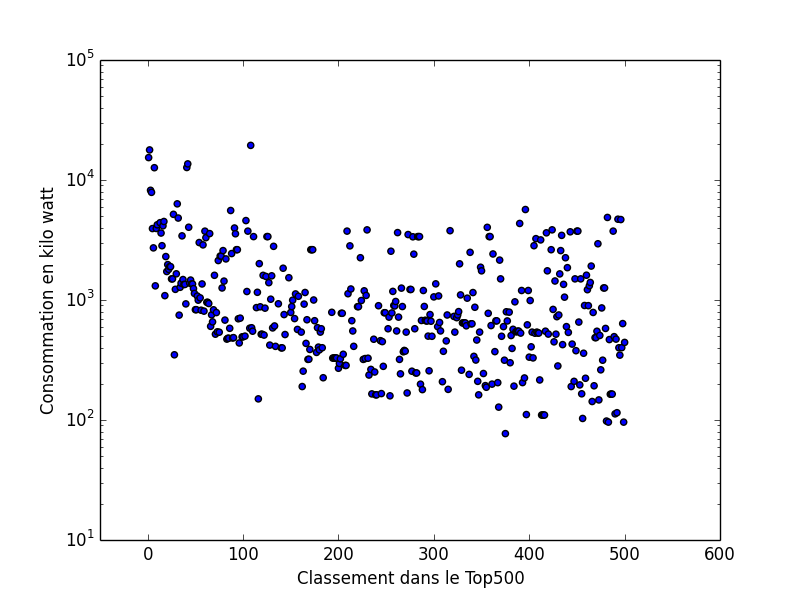
\includegraphics[width=10cm]{images/Chapitre1/pic_top500_power.png}
    \caption{\label{pic_top500_power} Consommation électrique des 500 supercalculateurs les plus puissants.}
\end{figure}



\subsubsection{Économique}
Le domaine du HPC est fortement influé par l'économie. En effet la construction de ces infrastructures coûte des millions d'euros d'investissement, et du fait que ces super-calculateurs sont des piliers stratégiques des entreprises, ces dernières sont très regardantes à leur coût. Cette forte pression de l'économie est une contrainte et il est difficile de proposer des sauts technologiques qui nécessitent de lourd investissement en amont sans connaître les retombés à l'avance. Comme vu dans la section consacré à l'énergie, nous devons repenser la façon dont nos codes sont conçus et exécutés. Par exemple en allant vers de nouvelles architectures comme les FPGA (Field Programmable Gate Array). Cette technologie permet de faire des périphériques très efficace en terme de consommation électriques. L'idée principale étant de laisser au programmeur le développement complet du circuit électronique pour qu'il corresponde parfaitement à son besoin. Mais la programmation de tels circuits est très complexe et demande des mois, souvent des années pour les codes complexes, pour être réalisée. Ainsi, malgré l'efficacité, prouvée, de cette technologie, les entreprises ne s'y lance pas à cause des coûts engendrés par les taille des équipes requises pour les programmer dans un temps raisonnable. On voit donc qu'il n'y a pas que les avancées et les nouvelles technologie qui sont importantes, il y a aussi leur facilité d'accès

\subsubsection{Technologiques}
Les différentes technologies connaissent elles aussi plusieurs contraintes. Une des principale à été exposé par Gordon Moore en 1965 qui a réalisé une conjecture qui est devenue la loi éponyme connus de tous. La loi de Moore prévoit que l'évolution du nombre de transistors sur une surface donnée va, grâce aux évolution technologique, être doublée tous les 2 ans à un prix constant. Sur la figure \ref{pic_Moore_prediction} on voit bien que cette évolution sur bel et bien la conjecture que le co-fondateur d'Intel a fait il y a plus de 50 ans.

\begin{figure}
    \center
    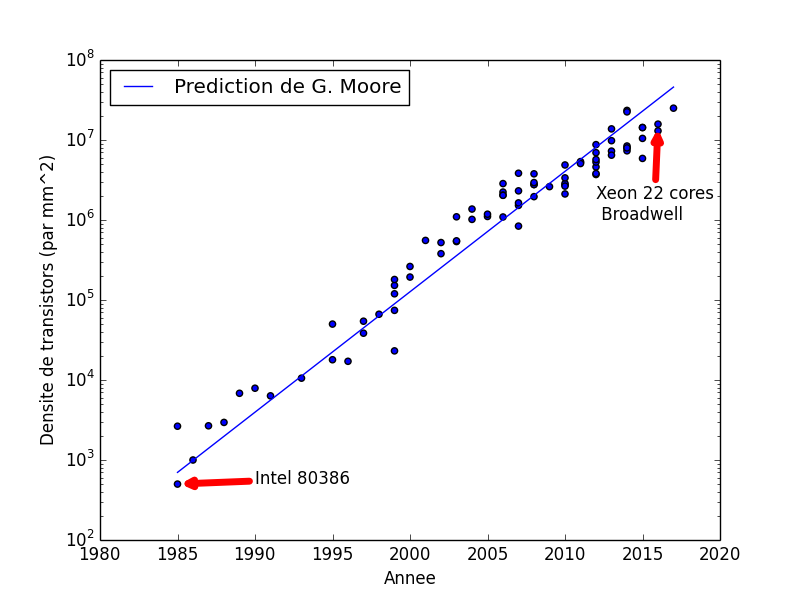
\includegraphics[width=10cm]{images/Chapitre1/Moore_prediction.png}
    \caption{\label{pic_Moore_prediction} La loi de Moore décrit l'évolution de la densité de transistors qui double tous les deux ans pour un prix constant (Données:  \url{https://en.wikipedia.org/wiki/Transistor_count}).}
\end{figure}


\textbf{TODO $Seminar_intro_v5.pdf$ slide 9 - expliquer moore par deux graphique: prix par mm2 et finesse de gravure}
Comme la puissance de calcul des processeurs est directement liée au nombre de transistors qu'ils contiennent, la puissance des puces à elle aussi suivi cette cadence. Alors pourquoi est ce devenu une contrainte ? Parce que pour doubler le nombre de transistors sans changer la surface gravée, il faut graver des transistors deux fois plus petits. Et si depuis 1965 on parvenait à le faire  au prix de nombreuses avancée techniques des appareils de gravure, nous atteignons aujourd'hui une limite physique, celle de la taille des atomes, voir figure \ref{pic_Moore_gravure}. En effet, aujourd'hui nous parvenons à graver des puces en autour de 10nm,  l'équivalent de quelques atomes. A cette taille les courants électriques ne sont plus stables et la course à la réduction des finesses de gravure est terminée. Alors qu'elle était un vecteur essentiel de l'évolution des performances, il va nous falloir trouver d'autres moyens pour arriver à atteindre l'exascale.

\textbf{TODO $Seminar_advanced technologies_v5.pdf$ slide 93 limite de Landauer}

\begin{figure}
    \center
    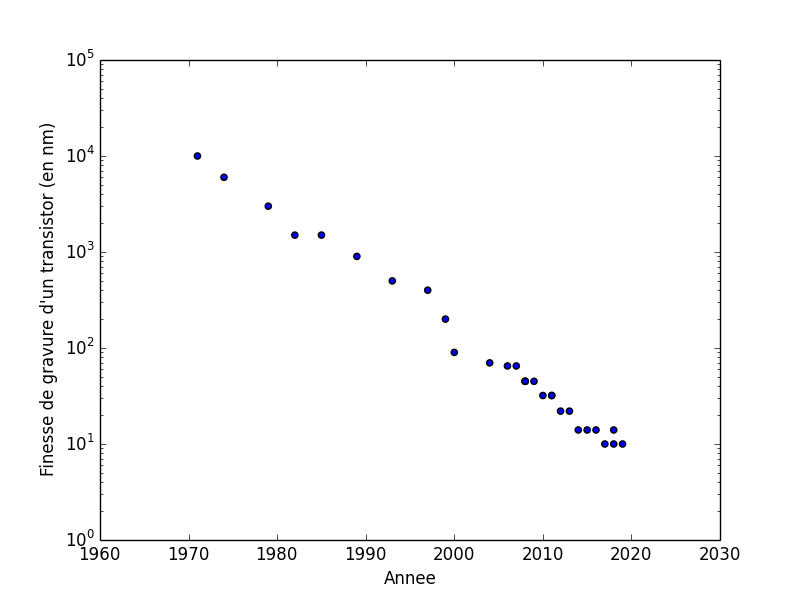
\includegraphics[width=10cm]{images/Chapitre1/Moore_gravure.png}
    \caption{\label{pic_Moore_gravure} La finesse des gravures à largement diminuée mais elle commence à toucher les limites de la physique \url{https://fr.wikipedia.org/wiki/Microprocesseur}).}
\end{figure}

La contrainte technique est très forte, d'autant plus avec l'apparition de nouvelles technologies plusieurs fois par ans. D'autant plus que souvent, ces nouveautés ne sont pas simplement des versions améliorées de précédents produits, ce sont souvent des technologies innovantes. Par exemple en c'est à partir de 2010 que l'on voit les premiers clusters contenant des cartes graphiques. Et il a fallut plusieurs années pour que cette technologie se fasse une place dans le monde du HPC notamment parce qu'elle nécessite une complète réécriture des codes. Il faut repenser la structure des algorithmes pour pouvoir tirer partie de tout le potentiel de ces cartes. Et il faut attendre 2013 pour voir une réelle percée de cette technologie (voir le graphique \ref{pic_GPU_repartition_TOP500}). Et il en est de même pour de nombreuses technologies innovantes, l'arrivée des mémoires non volatiles va demander aux utilisateurs de repenser une nouvelle fois leur algorithmes et seules des programmeurs expérimentés et avisés pourront le faire. L'exemple du FPGA est aussi un très bon exemple, sa complexité de programmation est un gros frein à son adoption. Et ces contraintes techniques se traduisent directement par un coût pour les entreprises. Car il faut engager des experts des différents domaines et investir de nombreuses heures pour faire les transformations adéquates.     


\begin{figure}
    \center
    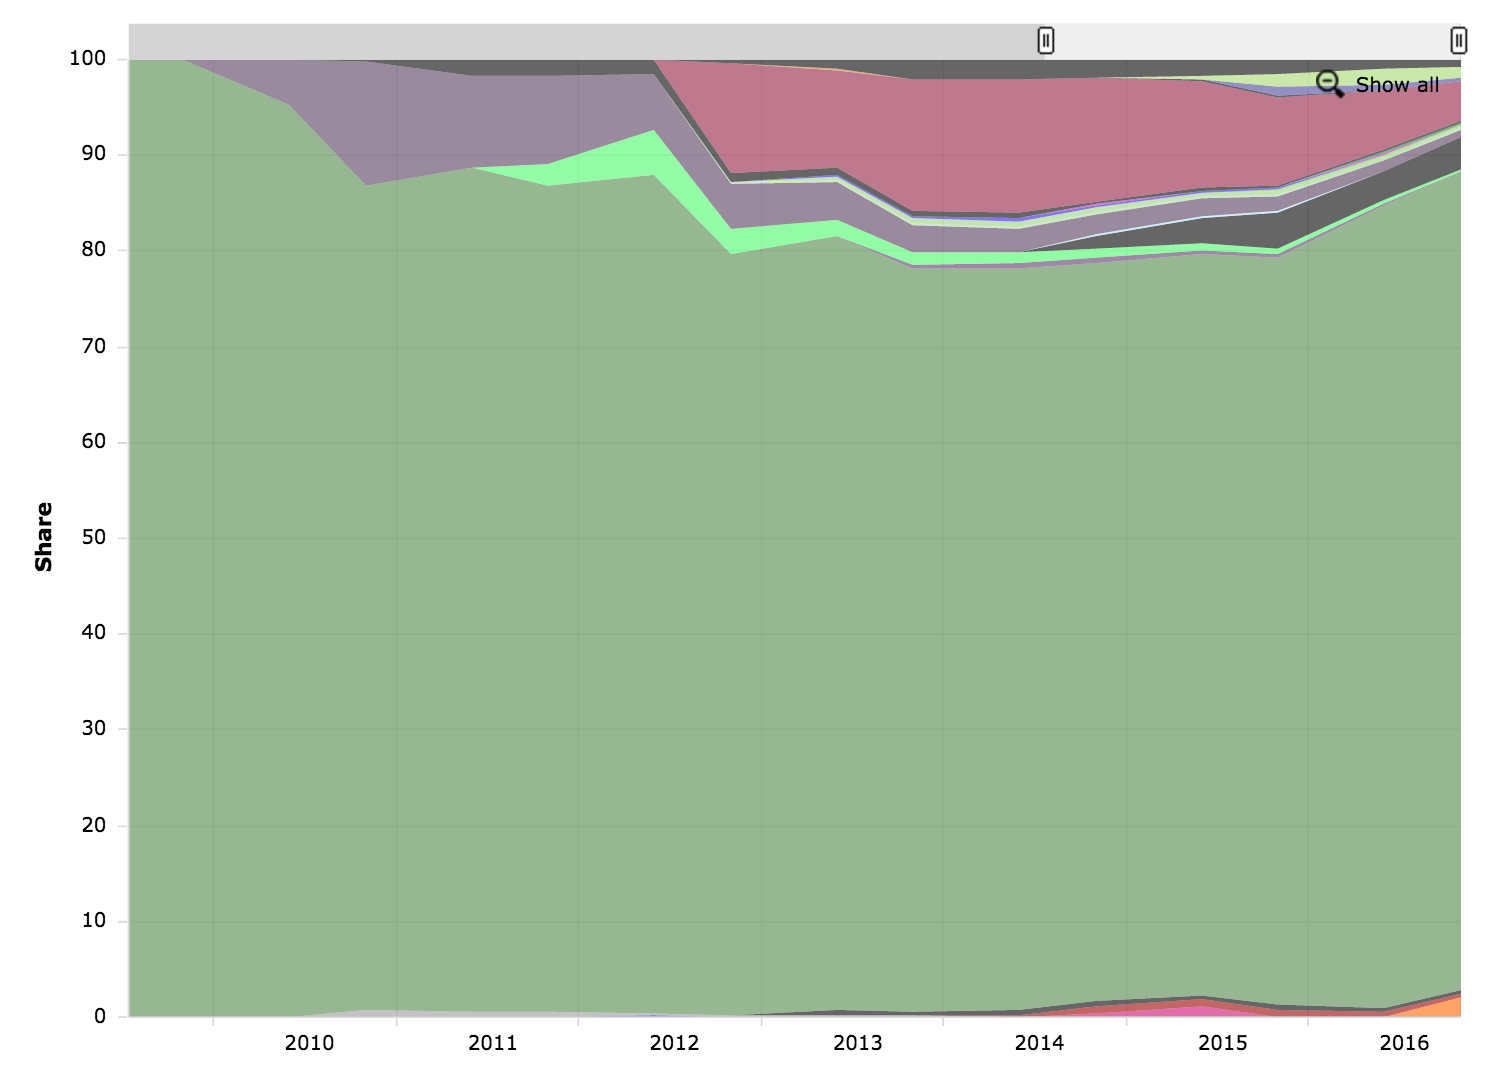
\includegraphics[width=10cm]{images/Chapitre1/pic_GPU_repartition_TOP500.png}
    \caption{\label{pic_GPU_repartition_TOP500} Partage de la performance totale du TOP500 entre les processeurs (couleur verte dominante) et les cartes graphiques (autres couleurs, représentants chaque modèles de cartes) \textit{source: \url{www.top500.org}}  }
\end{figure}

\subsubsection{Techniques et Connaissances}


Mes 3 ans d'expériences chez HPE et mon semestre de cours à Barcelone m'ont appris une chose: le domaine de l'analyse et des optimisations de performances est très difficile et nécessite de nombreuses connaissances et beaucoup d'expérience. La complexité des  architectures est telle qu'il est devenu impossible de prévoir avec précision leur comportement. Et ceci pour deux raisons: la première est le manque de connaissances fines de ces architectures et la deuxième est la faiblesse et la rareté des outils disponibles pour pour réaliser ce travail. En effet, pour contre balancer la complexité grandissante des architectures, il faut pouvoir utiliser des outils qui permettent de la comprendre. Or, la pauvreté des outils disponibles se fait ressentir et ceci pour une raison: personne n'en avait une réelle utilité jusqu'à maintenant. En réalité, il n'était pas nécessaire aux programmeurs de comprendre en détails toutes les finesses et toutes les particularités des architectures pour atteindre les performances voulues. Jusqu'à aujourd'hui il a suffit à l'industrie d'attendre les nouvelles versions des processeurs Intel (fameux modèle \textit{tic toc}) pour augmenter leur performances. Le travail d'optimisations ne valait alors pas le coup. C'est ainsi qu'aujourd'hui, alors que les contraintes se font plus pressantes que jamais, le domaine du HPC accuse le manques de développement d'outils et de formation de programmeur capable d'aller chercher ces performances.

De plus, les supercalculateurs se veulent de toujours plus hétérogènes en accueillant des accélérateurs diverses. Il faut donc calibrer les codes pour pouvoir être exécutés sur ces différentes architectures. Généralement, il faudra choisir un premier modèle de programmation dit à "mémoire distribuée". Il correspond à la partie du code qui s'occupe de partager le problème à résoudre entre les serveurs et qui s'occupe des communications. Le standard le plus utilisé celui de MPI (Message Passing Interface). Une fois le problème partagé, il faut coder le programme qui s'exécutera sur chaque serveurs, qui peuvent contenir plusieurs processeur. On utilise pour cela un deuxième paradigme de programmation, celui dit de "mémoire partagée". Enfin, ces serveurs peuvent aussi utilisé des accélérateurs (GPU, FPGA, DSP, etc.), il faudra donc écrire les programmes qui leur correspondent pour pouvoir les utiliser.
Les outils capables de nous aider dans ce travail nous manques et il est un objectif de cette thèse de fournir de tels outils. Mais il faut aussi user d'une méthodologie précise pour comprendre et optimiser ces codes. Fournir seulement un éventails d'outils ne sera pas suffisant si nous ne prodiguons pas les conseils que seule l'expérience peut apporter. Il est primordial de comprendre comment les codes sont exécutés sur nos système pour pouvoir espérer cibler de futures architectures comme \textit{The Machine}.



%%%%%%%%%%%%%%%%%%%%%%%%%%%%%%%%%%%%%%%%%%%%%%%%%%%%%%%%%%%%%%%%%%%%
%%%%%%%%%%%%%%%%%%%%%%%%%%%%%%%%%%%%%%%%%%%%%%%%%%%%%%%%%%%%%%%%%%%%
%%%%%%%%%%%%%%%%%%%%%%%%%%%%%%%%%%%%%%%%%%%%%%%%%%%%%%%%%%%%%%%%%%%%
%%%%%%%%%%%%%%%%%%%%%%%%%%%%%%%%%%%%%%%%%%%%%%%%%%%%%%%%%%%%%%%%%%%%
%%%%%%%%%%%%%%%%%%%%%%%%%%%%%%%%%%%%%%%%%%%%%%%%%%%%%%%%%%%%%%%%%%%%
%%%%%%%%%%%%%%%%%%%%%%%%%%%%%%%%%%%%%%%%%%%%%%%%%%%%%%%%%%%%%%%%%%%%
%%%%%%%%%%%%%%%%%%%%%%%%%%%%%%%%%%%%%%%%%%%%%%%%%%%%%%%%%%%%%%%%%%%%
%%%%%%%%%%%%%%%%%%%%%%%%%%%%%%%%%%%%%%%%%%%%%%%%%%%%%%%%%%%%%%%%%%%%
%%%%%%%%%%%%%%%%%%%%%%%%%%%%%%%%%%%%%%%%%%%%%%%%%%%%%%%%%%%%%%%%%%%%
%%%%%%%%%%%%%%%%%%%%%%%%%%%%%%%%%%%%%%%%%%%%%%%%%%%%%%%%%%%%%%%%%%%%
%%%%%%%%%%%%%%%%%%%%%%%%%%%%%%%%%%%%%%%%%%%%%%%%%%%%%%%%%%%%%%%%%%%%
%%%%%%%%%%%%%%%%%%%%%%%%%%%%%%%%%%%%%%%%%%%%%%%%%%%%%%%%%%%%%%%%%%%%
%%%%%%%%%%%%%%%%%%%%%%%%%%%%%%%%%%%%%%%%%%%%%%%%%%%%%%%%%%%%%%%%%%%%
%%%%%%%%%%%%%%%%%%%%%%%%%%%%%%%%%%%%%%%%%%%%%%%%%%%%%%%%%%%%%%%%%%%%
%%%%%%%%%%%%%%%%%%%%%%%%%%%%%%%%%%%%%%%%%%%%%%%%%%%%%%%%%%%%%%%%%%%%
%%%%%%%%%%%%%%%%%%%%%%%%%%%%%%%%%%%%%%%%%%%%%%%%%%%%%%%%%%%%%%%%%%%%
%%%%%%%%%%%%%%%%%%%%%%%%%%%%%%%%%%%%%%%%%%%%%%%%%%%%%%%%%%%%%%%%%%%%
%%%%%%%%%%%%%%%%%%%%%%%%%%%%%%%%%%%%%%%%%%%%%%%%%%%%%%%%%%%%%%%%%%%%

\section{Évolution des processeurs}

L'objectif de cette partie est de comprendre comment les architectures d'aujourd'hui sont devenues si complexes. Pour cela, nous allons étudier les évolutions technologiques chronologiquement pour comprendre en quoi elles étaient nécessaires et à quelle problématique elles répondent. Cet historique des ordinateurs bien que très complet n'aborde pas tous les points de ces architectures, mais seulement celles qu'il est important d'étudier pour comprendre l'état actuel de l'industrie.




%%%%%%%%%%%%%%%%%%%%%%%%%%%%%%%%%%%%%%%%%%%%%%%%%%%%%%%%%%%%%%%%%%%%
%%%%%%%%%%%%%%%%%%%%%%%%%%%%%%%%%%%%%%%%%%%%%%%%%%%%%%%%%%%%%%%%%%%%
\subsection{L'architecture}
Pour résoudre la multitudes de problèmes auxquels nous voulons apporté des réponses, nous utilisons des algorithmes. Pour écrire ces algorithmes on utilise des langages de programmation compréhensibles par un humain. Ces programmes sont alors lus par un programme appelé compilateur qui s'occupe de transformer le langage en un code compris seulement par le processeur qui lui pourra exécuter ces instructions. L'architecture de ces processeurs à beaucoup évolué depuis leur création, mais l'organisation globale n'a pas changé: la majorité des processeurs sont basés sur l'architecture \textit{Von Neumann}. C'est en 1945 que cette architecture à été présenté pour la première fois par John von Neumann dans un papier qu'il n'aura pas le temps de finir "First Draft of a Report on the EDVAC". Il y décrit une façon d'organiser un système électronique dans le but d'exécuter des instructions. La principale idée de cette architecture est la présence de 4 modules principaux:
 \begin{itemize}
    \item Une unité de traitement (CPU) qui contient une unité arithmétique et logique (ALU) qui s'occupe d'exécuter les opérations de bases (addition, multiplication, etc.) ainsi que de registres pour mémoriser les données utilisés pour leur exécutions
    \item L'unité de control qui lit les instructions et organise leur instructions en s'occupant de demander les données nécessaires à la mémoire.
    \item Une mémoire qui contient toutes les données nécessaires à l'éxécution du code mais aussi le code à éxecuter.
 \end{itemize}
 

 
 Dans ce papier il est précisé que la façon dont sont stocké le code à exécuter et les données en mémoires doit être la même contrairement à sa principale concurrentes, l'architecture  Harvard (figure \ref{pic_neumannHarvard}). Dans cette dernière, les instructions et les données sont stockées dans deux mémoires différentes et sont accédées par deux bus. Elles peuvent donc être accédées simultanément. Le problème de cette architecture vient des compilateurs qui souvent écrivent les données directement dans les instructions et les séparés n'a alors aucun interet. Aussi, la mémoire des instructions n'est accessible qu'en lecture rendant empêchant le programme de se modifier lui même ce qui est courant dans les codes (notamment du noyeau linux). Enfin la nécessité d'avoir deux bus rend les puces Harvard plus cher et les performances sont souvent moins bonnes. Un code qui aurait beaucoup d'accès mémoire ne pourrait pas profiter de la disponibilité du canal allant à la mémoire des instructions. Dans une architecture Von Neumann à deux canaux, les bus peuvent être utilisés aussi bien pour des instructions que pour les données.
 

\begin{figure}
    \center
    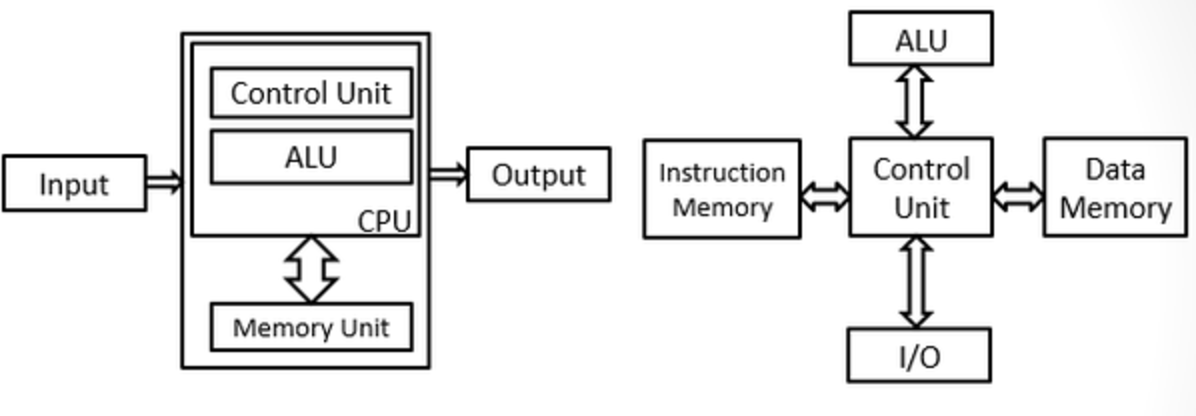
\includegraphics[width=10cm]{images/Chapitre1/neumannHarvard.png}
    \caption{\label{pic_neumannHarvard} Les deux principales architectures de processeurs: Von Neumann et Harvard. }
\end{figure}

Les architectures modernes des processeurs sont toujours construites sur ce modèle même si beaucoup de composants ont été ajoutés autour. L'architecture Von Neumann n'est capables de réaliser des calculs seulement avec les données présentes dans sa mémoire interne, les registres. Ainsi il faut charger les données présentes en mémoire jusque dans ces registres pour pouvoir effectuer les opérations. Et un problème majeur de cette architecture vient nous impacter très fortement 40 ans après sa création. En séparant ainsi la parti de calcul et la mémoire, le temps d'exécution d'un code est devenu très dépendant des liens qui relient ces deux parties. Ainsi, suite à de nombreuses avancés technologiques, les processeurs calcul 1000 fois plus vite qu'il ne faut de temps pour charger les données depuis la mémoire au processeur. Et les accès à la mémoire sont très fréquents comme on le voit sur la figure \ref{pic_Neumann}. Il faut charger les instructions à exécuter, charger les données nécessaires au calcul et enfin enregistrer le résultat. Ces liens sont donc très utilisés et sont devenus le  principal goulot d'étranglement, ou \textit{bottleneck} des applications. 



%%%%%%%%%%%%%%%%%%%%%%%%%%%%%%%%%%%%%%%%%%%%%%%%%%%%%%%%%%%%%%%%%%%%
%%%%%%%%%%%%%%%%%%%%%%%%%%%%%%%%%%%%%%%%%%%%%%%%%%%%%%%%%%%%%%%%%%%%
\subsection{Les instructions}
Un processeur exécute des instructions qui analysées par l'unité de traitement. Ces instructions sont en quelque sorte des mots appartenant à un langage que le processeur sait reconnaître. Pour que les programmes soient exécutables sur différentes architectures, il a fallu se mettre d'accord sur un langage à adopter, on appelle cela une ISA pour \textit{instruction set architecture}. Il existe deux familles d'ISA les jeux d'instrucions CICS pour \textit{Complex Instruction Set Computing} et les instructions RISC pour \textit{Reduced Instruction Set Computing}.

\subsubsection{CISC}  est la première famille d'instructions à avoir été utilisé massivement. Ces instructions sont dites complexes car une seule instructions peut à elle seule demander plusieurs opérations à réaliser. Par exemple une addition CISC s'occuperait de charger les données à la mémoire et d'exécuter l'addition ensuite. A l'origine beaucoup de codes étaient écrit en assembleur, et ce genre d'instructions permettaient au programmeur d'éviter d'écrire de nombreuses lignes de codes souvent redondantes. De plus les codes générés en CISC sont plus petit et nécessitent donc moins de mémoire, qui à l'origine manquait énormément.

\subsubsection{RISC} Le terme \textit{réduit} fait réference au nombre d'instructions plus petit que celles de CISC mais aussi pour signifier que le travail à réaliser par une instructions était moindre que pour une instruction CISC. En effet les instructions RISC sont exécutés en un seul cycles et correspondent à toutes les opération basiques que peut faire processeur. Pour réaliser une multiplications entre deux données, on devra alors explicitement charger la première donnée, puis la deuxième et enfin écrire l'instruction qui correspond à ma multiplication. Les instructions étant plus nombreuses le travail des compilateurs est augmenté mais souvent l'exécution des codes résultantes en est réduite. Les architectures nécessitent moins de transistors ce qui peut permettre d'augmenter le nombre de registres par exemple.

 Le RISC fut une réponse apporté a la lenteur de décodage du CISC et en 1970 John Cocke alors ingénieur chez IBM proposa de réduire le nombre d'instructions CISC et alors ont commencé à apparaitre des architectures RISC. En effet avoir des instructions complexes, même si rarement utilisées, augmente aussi la complexité de l'électronique utilisée pour les décoder. La philosophie du RISC est d'être rapide pour les cas communs d'utilisation et d'être le plus simple possible. Ces deux familles d'instructions ont toutes deux leurs avantages et leurs inconvénients et les puces actuelles comportent des parties qui executes du code en RISC et d'autres en CISC. L'ISA la plus rependu est le x86 qui se veut être un jeu d'instruction CISC. Le RISC augmente le nombre d'instructions lues séparément par le micro-processeur, si cela à le désavantage de consommer plus de mémoire, cela à aussi d'autre avantages, comme de pouvoir optimiser leur exécution avec la mise en place d'un \textit{pipeline}.
 
 \subsubsection{Le jeu d'instructions d'Intel: le x86} \textbf{TODO}
 
 
%%%%%%%%%%%%%%%%%%%%%%%%%%%%%%%%%%%%%%%%%%%%%%%%%%%%%%%%%%%%%%%%%%%%
%%%%%%%%%%%%%%%%%%%%%%%%%%%%%%%%%%%%%%%%%%%%%%%%%%%%%%%%%%%%%%%%%%%%
\subsection{Le pipeline } 
\label{sub_pipeline}
La chaîne de traitement du processeur, ou \textit{pipeline}, est une implémentation matériel d'un module qui permet de découper l'exécution d'une instructions en plusieurs étapes. Cette technique à pour effet de réduire drastiquement le nombre de cycles nécessaires à l'exécution d'un code. Le fait de partager l'exécution d'une instruction en sous étapes permet de commencer l'exécution de la suivante pendant que l'instruction actuelle est encore dans la chaîne d'exécution (voir figure ~\ref{pic_pipeline}).
\begin{figure}
    \center
    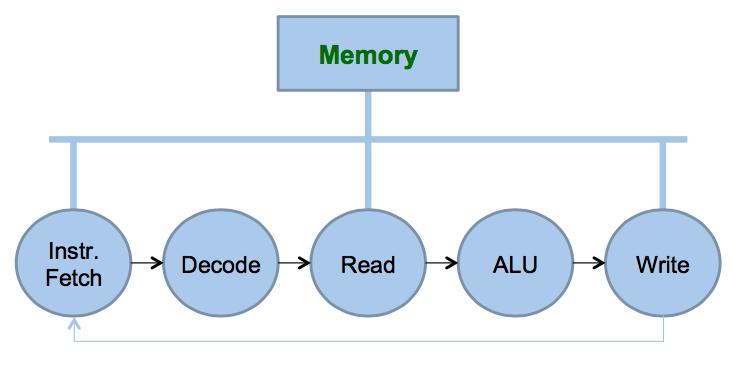
\includegraphics[width=10cm]{images/Chapitre1/Neumann.png}
    \caption{\label{pic_Neumann} Représentation simplifié d'un pipeline de 5 étapes.}
\end{figure}

 Il est commun de présenter la notion de pipeline avec un pipeline de 5 niveaux:

\begin{itemize}
    \item \textbf{Recherche de l'instruction} ou \textit{fetch}: cette première étape charge l'instruction à exécuter depuis la mémoire principale dans un registre du processeur. Grâce à un compteur interne, le registre \textit{Program Counter}, le processeur connaît l'adresse mémoire de la prochaine instruction à charger.
    \item \textbf{Décodage} ou \textit{décode}: une fois que l'instructions est chargé il faut la décoder pour déterminer quelle action il doit exécuter et quelles données sont nécessaires.
    \item \textbf{Execution} ou \textit{execute}: c'est durant cette étape que l'instruction est réellement exécuté. Suite au décodage le processeur peut réaliser plusieurs actions: utiliser l'ALU pour faire une opération, réaliser des mouvements de données ou déplacer l'exécution à une nouvelle adresse (branchement conditionnel ou \textit{branch})
    \item \textbf{Accès mémoire} ou \textit{memory}: lorsqu'une instructions est un acces mémoire (\textit{load} ou \textit{store}), c'est durant cet étape qu'il est réalisé.
    \item \textbf{Ecriture du résultat} ou \textit{write back}: Enfin le processeur doit enregistrer le résultat produit par l'étape \textit{execute}. Si c'est un branchement, il modifie le registre PC, si c'est une opération arithmétique il sauvegarde le résultat dans l'adresse destinataire.
\end{itemize}

On peut par exemple commencer à charger la prochaine instruction (étape \textit{fetch}), alors que l'instruction actuelle est en train d'être exécutée (étape \textit{execute}). Sur la figure \ref{pic_pip_yes} on assiste à l'exécution de 5 instructions, au premier temps un seul instruction est exécutée, à l'étape $IF$ pour \textit{instruction fetch}. Ensuite (ligne suivante) une nouvelle instruction est chargé (opération $IF$) pendant que la première est passé à l'étape suivante (opération $ID$). Ainsi au bout de 5 cycles, chaque étape du pipeline est utilisée (partie en verte). 



\begin{figure}[t!]
    \begin{subfigure}[t]{0.5\textwidth}
        \centering
        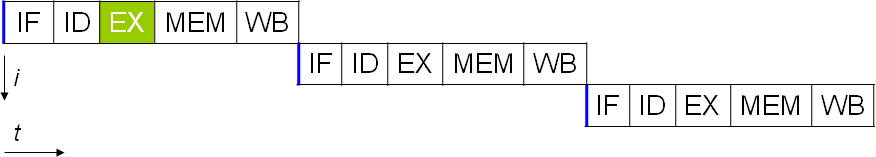
\includegraphics[height=0.4in]{images/Chapitre1/pipelineNo.png}
        \label{pic_pip_no}
        \caption{Processeur sans pipeline}
    \end{subfigure}%
    \begin{subfigure}[t]{0.5\textwidth}
        \centering
        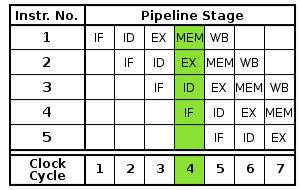
\includegraphics[height=0.7in]{images/Chapitre1/pipelineYes.png}
        \caption{Processeur avec un pipeline à 5 étages}
        \label{pic_pip_yes}
    \end{subfigure}
    
    \caption{Pipeline: en séquençant les instructions le processeur est capable d'exécuter des étapes différentes en parallèles (\textit{IF: instruction fetch, ID: instruction decode, EX: execution, MEM: memory, WB: write back}). Le nombre de cycle necessaire pour l'exécution passe alors de 25 à 9 cycles pour exécuter 5 instructions (source: \url{https://fr.wikipedia.org/wiki/Pipeline_(architecture_des_processeurs)} }
    \label{pic_pipeline}
\end{figure}





En 1939 IBM conçoit le premier processeur avec pipeline. Ce n'est qu'en 1989 qu'Intel produira le siens. Le nombre d'étapes, ou profondeur du pipeline, était de 2 à l'origine et a augmenté au fil du temps atteignant 31 étapes pour l'architecture du Pentium 4 Prescott d'Intel en 2004. Mais l'agrandissement du pipeline n'est pas gratuite, en effet, une chaîne de traitement plus grande prendra plus de place sur la puces et consommera plus d'énergie. Sur la figure \ref{pic_pipeline_evo} on voit que la consommation électrique a freiné l'évolution de la taille du pipeline.


 \begin{figure}
    \center
    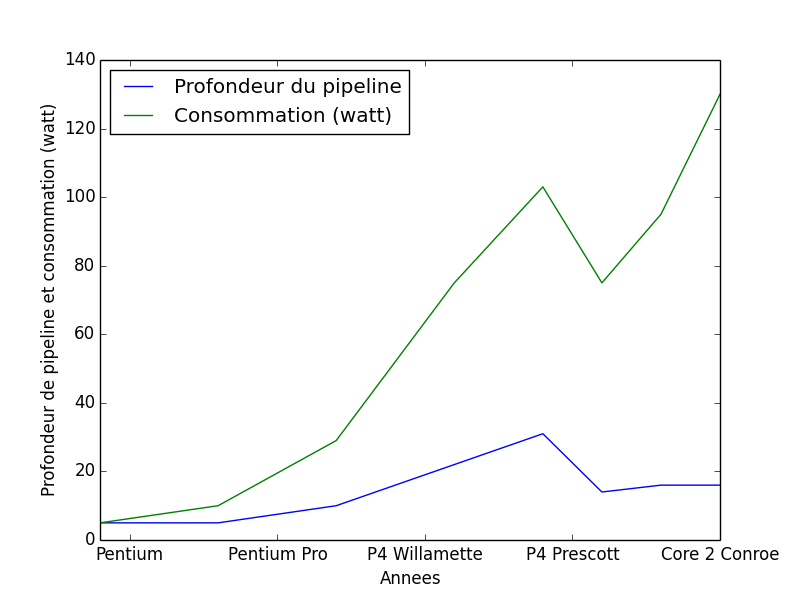
\includegraphics[width=7cm]{images/Chapitre1/pipeline_evo.png}
    \caption{\label{pic_pipeline_evo} L'évolution de la taille du pipeline des processeurs influe sur la consommation électrique}
\end{figure}

L'implémentation du pipeline à aussi ouvert la porte a de nombreuse optimisations. Ici sont présentés les avancées majoritaires qui vont impacter notre stratégie d'optimisation des codes.

\subsubsection{Pré-extraction - prefetch}

\begin{fancyquotes}
La pré-extraction est une technique efficace d'accès aux donnés qui permet de masquer l'attente du processeur quand une donné lui manque et pour diminuer la différence de performance entre les processeur et les mémoires. \cite{Byna2009}
\end{fancyquotes}

Un des défis des processeur est de réduire au maximum l'attente de donnés en provenances de la mémoire. Après avoir chargé la donné le processeur la décode, s'il a besoin d'une donnée pour réaliser un calcul par exemple il la demande à la mémoire. Un processeur sans \textit{prefetch} chargerait la donnée à chaque fois qu'il se rend compte qu'il en a besoin et comme les accès aux données prennent plusieurs cycles (voir centaines), il doit attendre que la donnée soit chargée dans un registre pour pouvoir l'utiliser. Le principe du \textit{prefetch} est d'anticiper cette demande et de charger la donnée avant même qu'elle soit demandée pour que lorsque le processeur en aura besoin, la donnée soit déjà chargée dans un registre.
Les instructions ou les données sont stockées en mémoires de façon continue. Ainsi les adresses des instructions qui sont exécutées auront tendances à se suivre. De même pour les données, les algorithmes ont tendances à travailler sur des structures de données comme les tableaux, et à les parcourir de façon continue ou avec un motifs (une case sur deux par exemple). L'optimisation apportée par le \textit{prefetch} permet de cacher cette latence incombée par la lenteur des mémoires. Si un code accède de façon méthodique à un tableau, le processeur va détecter ce motifs grâce à un composant dont la responsabilité est de détecter de tels motifs. Il va donc permettre d'anticiper les accès mémoire pour charger les données avant qu'elles ne soient utilisées. Ce système est très puissant car la latence de centaines de cycles de la mémoire peut être cachée par cette technique. Cependant, même les processeurs les plus modernes ne détecte pas tous les motifs d'accès. Par exemple si on parcourt un tableau une case sur 4, certains processeurs ne seront pas capable de détecter ce motif\textbf{TODO A VERIFIER}. Il est donc très important que le programmeur soit sensibilisé à cette fonctionnalité pour pouvoir en tirer partie en ajustant les motifs d'accès aux données ou bien à la façon dont elles sont stockées.
Il y a deux façon d'activer le prefetching. La première exposée précédemment est faite de façon autonome par un composant du processeur qui essaie de trouver des motifs d'accès logiques appelé le \textit{hardware prefetch}. Le second moyen de l'activer est de le faire de façon logiciel, \textit{software prefetch}. Ainsi, le programmeur lui même, ou le compilateur ajoute des instructions dans le code pour réaliser les requêtes mémoires à l'avance.

\textbf{TODO exemple de software prefetching p61}

\subsubsection{Execution dans le désordre - Out of order}
\begin{fancyquotes}
Ne pas attendre l'exécution d'une instruction précédente si cette instruction n'en dépend pas. %\cite{out_of_order:online}
\end{fancyquotes}
Comme pour le \textit{prefetch}, le but de cet optimisation est de cacher l'attente de donnée du processeur de la mémoire. Cette avancée est apparue sur les processeurs Itel en 1995 avec le \textit{pentium P6}. Le principe de l'exécution dans le désordre est d'exécuter les instructions dans un ordre différent que celui donné par le code source.  Ainsi lorsqu'une instruction doit attendre une donnée, au lieu de perdre des cycles inutilisé à attendre ces données. Le processeur va executer les instructions qui suivent et finira d'exécuter la première quand la donné sera chargée dans un registre. Cependant ne pas exécuter le programme dans l'ordre initial peut fausser les résultats. C'est alors au processeur de s'assurer que les instructions permutées ne sont pas dépendantes. Il existe trois types de dépendances:
\begin{itemize}
    \item Read after Write: une instruction lit une donnée écrite par une instruction la précedent.
    \item Write after Read: une première instruction lit une donnée qui est modifiée par une instruction la suivant.
    \item Write after Write: deux instructions écrivent sur la même donnée. 
\end{itemize}



\begin{lstlisting}[language=C, caption=Exemples de dépendances entre deux instructions., float,floatplacement=H, label=code_dependances]
//----------- Read after Write -----------
int A, B = 0
A = 5;
B = A + 10;
//Result: B == 10 ou B == 15

//----------- Write after Read -----------
int A, B = 0
B = A + 10;
A = 5;
//Result: B == 10 ou B == 15 
 
//----------- Write after Write -----------
int B = 0
B = 5;
B = 10;
//Result: B == 5 ou B == 10
\end{lstlisting}


L'extrait de code \ref{code_dependances} donne un exemple pour chaque type de dépendances. Dans chaque cas, la valeur de B n'est pas la même si les deux assignations ne sont pas exécutées dans le même ordre, suivant cet ordre, B peut valoir 10 ou 15. Pour ce faire, le processeur possède une fenêtre de plusieurs instructions, aussi appelée (à tord) l'\textit{execution queue}. En effet, cette liste n'a pas vocation à être executé dans l'ordre, c'est un rassemblement d'instructions qui ont des dépendances entre elles. Le processeur vient mettre à jour cette liste pour essayer d'exécuter des instructions qui n'ont pplus de dépendances avec une donné ou une autre instruction.
Pour pouvoir bénéficier de l'exécution dans le désordre, le processeurs doit donc détecter si les instructions sont dépendantes pour pouvoir les réordonner. Aussi, le programmeur peut aider le processeur dans son travail en évitant au maximum les dépendances entre les instructions. 

\subsubsection{TODO Register renaiming ?}


\subsubsection{TODO Branch Prediction ?}



%%%%%%%%%%%%%%%%%%%%%%%%%%%%%%%%%%%%%%%%%%%%%%%%%%%%%%%%%%%%%%%%%%%%
%%%%%%%%%%%%%%%%%%%%%%%%%%%%%%%%%%%%%%%%%%%%%%%%%%%%%%%%%%%%%%%%%%%%
\subsection{La Floating Point Unit (FPU)}

L'unité de calcul en virgule flottante (FPU pour \textit{floating-point  unit}) est un composant du processeurs permettant de réaliser les opérations sur les nombres à virgule flottante. A l'origine ce module était séparé du processeur et il convenait à l'utilisateur de choisir si il voulait ou non en brancher une sur la carte mère dans l'emplacement qui lui était alors dédié. Pour des questions de coûts d'intégration et de performance, la FPU est depuis 1989, avec la sortie du processeur Intel 80486,  intégrée au processeur. 

Au fil des années la complexité de la FPU a augmenté, quand elle n'était capable d'exécuter que de simples opérations à l'origine, elle peut désormais réaliser des opérations complexes (division, racine carrée, exponentielles ou des fonctions trigonométriques).  De plus, des instructions fusionnées ont fait leur apparition en 2013 dans les processeurs \textit{Haswell} de Intel et Piledriver pour AMD. Elles ont la particularité de réaliser 2 opérations en un seul cycle d'horloge du processeur. Connues sous le nom de FMA pour \textit{fused multiply-add} elles sont capables d'exécuter l'instruction $a \leftarrow b * c + d$ en un seul cycle. 

Enfin, les unités de calcul modernes sont capable d'exécuter une opération sur plusieurs données à la fois ce type d'instructions est dit \textit{vectoriel}. Ces instructions sont performantes pour les algorithmes qui doivent exécuter une même opération sur plusieurs données (un vecteur par exemple). L'évolution de leurs caractéristiques sont abordées dans la partie \ref{sub_taxonomie}.
Les différentes évolution de la FPU sont responsable de la forte augmentation de la puissance de processeur. En effet, usuellement la puissance d'un processeur est donnée par le nombre de calculs flottant qu'il peut exécuter par cycle. Le tableau \ref{tab_FPU} montre comment le nombre de FLOP par cycle évolue: Pour Intel, cette performance a été multipliée par deux à chaque nouvelle version de l'architecture et les FPU modernes exécutent 8 fois plus de calculs qu'en 2008.

\begin{table}[]
\centering
\caption{Evolution de la performance des FPU}
\label{my-label}
\begin{tabular}{|l|l|l|l|l|l|}
\hline
\multicolumn{1}{|c|}{\textbf{Année}} & \multicolumn{2}{c|}{\textbf{Architecture Intel / AMD}}     & \multicolumn{1}{c|}{\textbf{Simpe p.}} & \multicolumn{1}{c|}{\textbf{Double p.}} & \multicolumn{1}{c|}{\textbf{Opérations}} \\ \hline
2008                                 & Nehalem                          & K10                     & 8                                      & 4                                       & 4 add. et 4 mul.         \\ \hline
2011                                 & Sandy Bridge                     & Bulldozer               & 16                                     & 8                                       & 8 add. et 8 mul.         \\ \hline
2013                                 & Haswell \& Skylake               &                         & 32                                     & 16                                      & 8 FMA (mult. + add.)        \\ \hline
2016                                 & Xeon Phi KNL &                         & 64                                     & 32                                      & 8 FMA (mult. + add.)        \\ \hline
\end{tabular}
\label{tab_FPU}
     \vspace{1ex}

     \raggedright Avec Haswell le nombre d'instructions exécutable n'évolue pas mais c'es le type d'instructions exécuté qui sont des FMA (une multiplication et une addition en un cyle d'horloge) et qui correspond à deux FLOP.
\end{table}

\textbf{TODO} latence des differentes instructions; skylake FMA 4 cycles %http://agner.org/optimize/blog/read.php?i=415 (calc_fma() combien de FMA en parallele)


%%%%%%%%%%%%%%%%%%%%%%%%%%%%%%%%%%%%%%%%%%%%%%%%%%%%%%%%%%%%%%%%%%%%
%%%%%%%%%%%%%%%%%%%%%%%%%%%%%%%%%%%%%%%%%%%%%%%%%%%%%%%%%%%%%%%%%%%%
\subsection{Processeur super-scalaire}
\begin{fancyquotes}
On appelle \textit{super-scalaire} un processeur capable d'exécuter plus d'une instruction par cycle d'horloge. \cite{smith1995microarchitecture}
\end{fancyquotes}
Les premiers processeurs disposant de cette optimisations ont été produit entre 1988 et 1990 par Motorola, Intel et AMD. Intel produira le premier processeur super-scalaire utilisant des instructions x86 en 1993 avec le \textit{Pentium P5}. Grâce au passage d'instructions CISC à RISC, la complexité des micro-processeurs a diminuée permétant d'intégrer de nouvelles fonctionnalités. Une architeture super-scalaire à pour objectif d'augmenter la performance du pipeline en construisant des processeurs avec plusieurs pipelines. Cependant, comme pour le principe de l'\textit{out-of-order}, il faut que le processeur ait a sa disposition des instructions qui indépendantes. Un processeur à plusieurs pipeline voit donc les unités présentées dans la section \ref{sub_pipeline} démultipliées.  Ainsi le processeur peut décoder plusieurs instructions, charger les données en parallèles et améliorer l'utilisation des unité d'exécution (comme la FPU). Le graphique \ref{pic_superscalar} montre un exemple de processeurs à deux pipeline. Chaque étapes de traitement a été dédoublée et le processeur peut maintenant executer, au maximum, 2 instructions par cycles d'horloges. A titre de comparaison un processeur Intel Haswell (2013) possède 8 files d'exécutions et peut exécuter jusqu'à 4 opérations flottantes par cycle.

\begin{figure}
    \center
    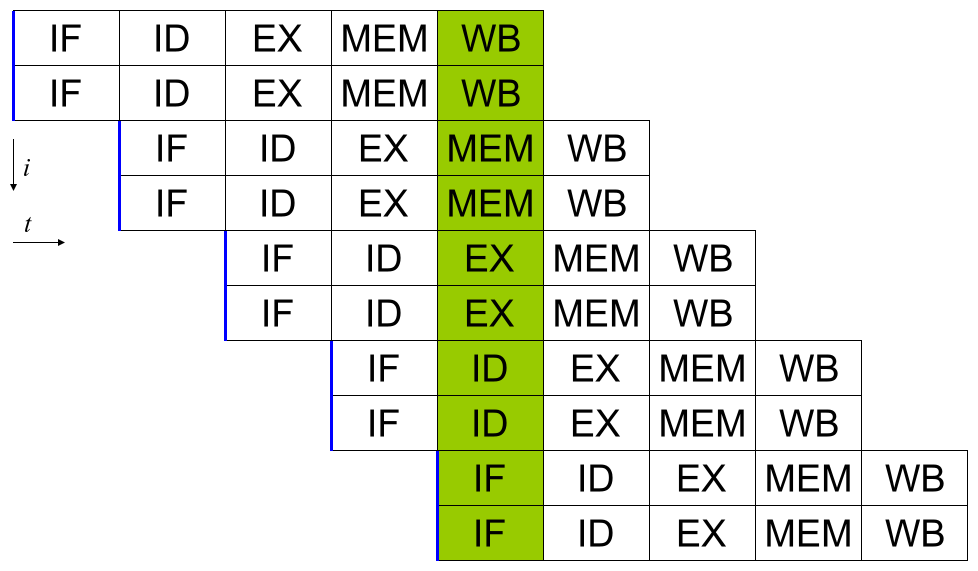
\includegraphics[width=7cm]{images/Chapitre1/superscalar.png}
    \caption{\label{pic_superscalar} Exemple d'un processeur a 2 pipeline (source \url{https://en.wikipedia.org/wiki/Superscalar_processor}) }
\end{figure}

Executer plus d'une instruction par cycle
Cool si on arrive a apport des instructions indépendantes
Exemple du sandy bridge these papier
PAr exemple requete memoire en meme temps que un calcul

Programmer: donner un exemple de si on interlive un code ou non (PAtrick ? ) ou celui page 21














%%%%%%%%%%%%%%%%%%%%%%%%%%%%%%%%%%%%%%%%%%%%%%%%%%%%%%%%%%%%%%%
%%%%%%%%%%%%%%%%%%%%%%%%%%%%%%%%%%%%%%%%%%%%%%%%%%%%%%%%%%%%%%%
\subsection{Processeur vectoriel}
\begin{fancyquotes}
Un processeur vectoriel travaille sur un groupe de données indépendantes Les opérandes sont alors stockées dans des registres vectoriels capable de charger un vecteur pour y appliquer une même opération \cite{hughes2015single}
\end{fancyquotes}

 En effet dans les années 90, les ordinateurs personnels commencés à être utilisé pour lire des vidéos ou de la musique. Dans le but d'augmenter la performance de ces applications multimédia mais aussi d'augmenter les performances des processeurs tout en ne consommant pas plus d'énergie les architectes ont voulu améliorer l'efficacité d'une instruction en implémentant des architectures SIMD (\textit{Single Instruction Multiple Data} de la taxonomie de Flynn \label{sub_taxonomie}).Le principe est d'exécuter une instruction non pas sur une donnée comme le font les processeurs dit scalaires, mais sur un ensemble de données communément appelées vecteur (figure \ref{pic_simd}).
 
 

\begin{figure}
    \center
    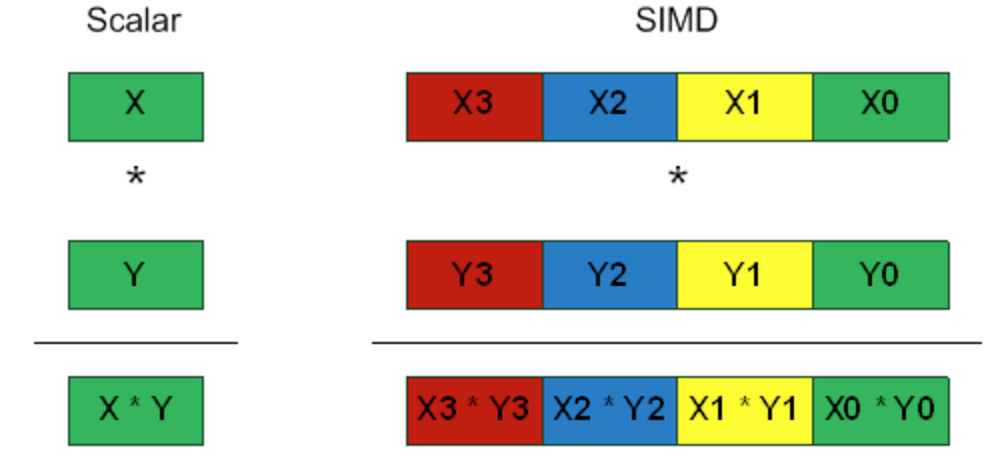
\includegraphics[width=7cm]{images/Chapitre1/simd.png}
    \caption{\label{pic_simd} Schéma de fonctionnement d'une multiplication vectorielle (\url{https://software.intel.com/en-us/articles/ticker-tape-part-2}}
\end{figure}

 
 C'est en 1995 que Sun Microsystem introduit son premier jeu d'instruction vectoriel, le \textit{Visual Instruction Set} auquel Intel répondra en 1997 avec son processeur Pentium MMX et son jeu d'instructions du même nom. Ainsi ces instructions pouvaient réaliser des opérations sur les jeux de données tel que les images ou vidéos de façon très performante. En 1997 AMD viendra améliorer le jeu d'instruction MMX avec l'implémentions des instructions \textit{3DNow!} qui rendait alors possible les opérations vectoriels sur les nombre flottant. La possibilité de faire une opération sur deux nombre flottant par cycle doublait alors la performance des processeurs. Intel répondit alors à cette avancé avec le jeu d'instructions Streaming SIMD Extensions (SSE) en 1999. Il est alors facile d'augmenter la puissance des processeurs: il suffit d'augmenter la taille des vecteurs. Au plus ils pourront appliquer les instructions sur de données, au plus grand sera le nombre de FLOP par cycle réalisés. Les versions suivantes des jeu d'instructions vectorielles ne feront que continuer dans ce sens en utilisant des processeurs avec plus de registres vectoriels mais aussi de taille plus grande (voir \ref{tab_simd}).
 
 
 

\begin{table}[]
\centering
\caption{Évolutions principales des instructions SIMD de $x86$}
\label{tab_simd}
\begin{tabular}{|l|l|l|l|l|l|}
\hline
\multicolumn{1}{|c|}{\textbf{Année}} & \multicolumn{1}{c|}{\textbf{Nom}} & \multicolumn{1}{c|}{\textbf{Nb registres}} & \multicolumn{1}{c|}{\textbf{Taille (bit)}} & \multicolumn{1}{c|}{\textbf{Registres}} & \multicolumn{1}{c|}{\textbf{Commentaires}} \\ \hline
1996                                 & MMX                               & 8                                          & 64                                         & MM0                                     & Nombre entiers
\\ \hline
1999                                 & SSE                               & 8                                          & 128                                        & XMM0                                    & 120 instr., simple precisions              \\ \hline
2006                                 & SSSE3                             & 8                                          & 128                                        & XMM0                                    & 300 instr., double précisions              \\ \hline
2008                                 & AVX                               & 16                                         & 128                                        & XMM0                                    & FMA4, op. a 3 opérandes                    \\ \hline
2011                                 & AVX2                              &  16                                          & 256                                        & YMM0                                    &                                            \\ \hline
2013                                 & AVX512                            & 32                                         & 512                                        & ZMM                                     & FMA3                                       \\ \hline
\end{tabular}
\end{table}

\begin{figure}
    \center
    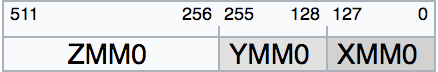
\includegraphics[width=7cm]{images/Chapitre1/simd_registres.png}
    \caption{\label{pic_simd_registres} Découpage d'un registre de 512 bits}
\end{figure}


 Aussi, utiliser des instructions vectorielles permet de s'assurer que la bande passante utilisé l'est pour des données utiles. A la différence d'instruction scalaire ou le processeur doit charger une \textit{cache line} avec des données pas toujours utiles, utiliser des instructions vectorielles force le développeur à repenser ses structures de données.


Cependant, dans la pratique les codes ne sont pas aussi parallèle que nous le souhaiterions et certains aspect du code empêche de tirer la totalité de la performance disponible. En effet, si les données sont indépendantes les unes des autres, il est alors impossible de les calculer simultanément rendant la partie vectorielle inutilisable. Aussi les performances peuvent  être réduites si les données accédées ne sont pas continues en mémoire.  Cela demande donc un travail supplémentaire pour repenser les structures de données et s'assurer que les donnés transférées sur le bus mémoire sont des données \textit{utiles} (voir le concept de ligne de cache TODO ref). Par exemple le calcul vectoriel ne s'appliquera pas sur une structure de données irrégulière comme un tableau de \textit{structures}. Enfin, cette amélioration réduit la pression que subit l'unité responsable du \textit{fetch} et du \textit{decode}. Car avec une seule instruction vectorielle, le processeur réalise le travaille de plusieurs instructions scalaires qui n'auront pas besoin d'être décodées. Il en résulte que doubler largeur des instructions revient à doubler le nombre de FLOP réalisable par le processeur alors que la consommation électrique augmentera d'un facteur inférieur à 2. Beaucoup d'efforts ont donc été réalisé pour être capable d'utiliser cette technologie, par exemple la majorité des compilateurs est capable de détecter les zones de codes parallélisable pouvant bénéficier d'instructions SIMD.





%%%%%%%%%%%%%%%%%%%%%%%%%%%%%%%%%%%%%%%%%%%%%%%%%%%%%%%%%%%%%%%%%%%%
%%%%%%%%%%%%%%%%%%%%%%%%%%%%%%%%%%%%%%%%%%%%%%%%%%%%%%%%%%%%%%%%%%%%
\subsection{Processeur multi-cœur}
2000 Netburst architecture - 2000
The architecture of modern CPUs is largely dictated by the fact that getting data from memory is much
slower than processing it. Hence, a hierarchy of ever faster and smaller tries to keep data as close to the
processing unit as possible, mitigating the long latency and small bandwidth of main memory. The ILP in
the processing unit also helps to hide the latency and more fully utilize the available bandwidth.

%%%%%%%%%%%%%%%%%%%%%%%%%%%%%%%%%%%%%%%%%%%%%%%%%%%%%%%%%%%%%%%%%%%%
%%%%%%%%%%%%%%%%%%%%%%%%%%%%%%%%%%%%%%%%%%%%%%%%%%%%%%%%%%%%%%%%%%%%
\subsubsection{Intel Hyperthreading \copyright}

Hyperthreading, on the other hand, refers to a very specific hardware technology created by Intel, which allows a single processor core to interleave multiple threads of execution more efficiently. In other words, a CPU with hyperthreading is going to provide performance which is somewhat greater than a CPU which is otherwise the same but without hyperthreading, because the hyperthreaded CPU will be able to concurrently balance two (sometimes more, but hyperthreading is usually 2-way) threads of execution on a given core.

Hyper-threading enables a single processor core to be used for two or more concurrent executions with just a little extra hardware.

 

%%%%%%%%%%%%%%%%%%%%%%%%%%%%%%%%%%%%%%%%%%%%%%%%%%%%%%%%%%%%%%%%%%%%
%%%%%%%%%%%%%%%%%%%%%%%%%%%%%%%%%%%%%%%%%%%%%%%%%%%%%%%%%%%%%%%%%%%%
\subsection{Multiprocesseur symétrique (SMP) }
2006 Core architecture
Les system équipé de processeurs identiques.

\subsubsection{Lien QPI}
\subsubsection{NUMA}
2006 Core Architecture



%%%%%%%%%%%%%%%%%%%%%%%%%%%%%%%%%%%%%%%%%%%%%%%%%%%%%%%%%%%%%%%%%%%%
%%%%%%%%%%%%%%%%%%%%%%%%%%%%%%%%%%%%%%%%%%%%%%%%%%%%%%%%%%%%%%%%%%%%
\subsection{Les fréquences}
\subsubsection{Turbo}
2011 Sandy Bridge Architecture
	Turbo Boost

At the same time, the focus on uniprocessor performance was shifting to clock speed. In the mid-to-late 1990s clock frequency increases in general-purpose processors accelerated dra matically. Manufacturers of desktop processors oftencompeted directly on clock frequency rather than actual performance. For programmers, this was fantastic—getting much better performance automatically across generations meant less effort was needed on code optimization. However, this was short-lived. In the early 2000s, this clock frequency war ended rather abruptly as pro cessor designers were reined in by physical constraints—clock frequency increases had drastically increased processor power consumption, and this was stressing cooling technology, not to men tion battery life of the increasingly important laptops.

%%%%%%%%%%%%%%%%%%%%%%%%%%%%%%%%%%%%%%%%%%%%%%%%%%%%%%%%%%%%%%%%%%%%
%%%%%%%%%%%%%%%%%%%%%%%%%%%%%%%%%%%%%%%%%%%%%%%%%%%%%%%%%%%%%%%%%%%%
\subsection{Les accélérateurs}
Creation de processeur spécific a certains besoins

\subsubsection{PCI Express}

\subsubsection{GPU}

\subsubsection{FPGA}


%%%%%%%%%%%%%%%%%%%%%%%%%%%%%%%%%%%%%%%%%%%%%%%%%%%%%%%%%%%%%%%%%%%%
%%%%%%%%%%%%%%%%%%%%%%%%%%%%%%%%%%%%%%%%%%%%%%%%%%%%%%%%%%%%%%%%%%%%
%%%%%%%%%%%%%%%%%%%%%%%%%%%%%%%%%%%%%%%%%%%%%%%%%%%%%%%%%%%%%%%%%%%%
%%%%%%%%%%%%%%%%%%%%%%%%%%%%%%%%%%%%%%%%%%%%%%%%%%%%%%%%%%%%%%%%%%%%
%%%%%%%%%%%%%%%%%%%%%%%%%%%%%%%%%%%%%%%%%%%%%%%%%%%%%%%%%%%%%%%%%%%%
%%%%%%%%%%%%%%%%%%%%%%%%%%%%%%%%%%%%%%%%%%%%%%%%%%%%%%%%%%%%%%%%%%%%
%%%%%%%%%%%%%%%%%%%%%%%%%%%%%%%%%%%%%%%%%%%%%%%%%%%%%%%%%%%%%%%%%%%%
%%%%%%%%%%%%%%%%%%%%%%%%%%%%%%%%%%%%%%%%%%%%%%%%%%%%%%%%%%%%%%%%%%%%
%%%%%%%%%%%%%%%%%%%%%%%%%%%%%%%%%%%%%%%%%%%%%%%%%%%%%%%%%%%%%%%%%%%%
%%%%%%%%%%%%%%%%%%%%%%%%%%%%%%%%%%%%%%%%%%%%%%%%%%%%%%%%%%%%%%%%%%%%
%%%%%%%%%%%%%%%%%%%%%%%%%%%%%%%%%%%%%%%%%%%%%%%%%%%%%%%%%%%%%%%%%%%%
%%%%%%%%%%%%%%%%%%%%%%%%%%%%%%%%%%%%%%%%%%%%%%%%%%%%%%%%%%%%%%%%%%%%
%%%%%%%%%%%%%%%%%%%%%%%%%%%%%%%%%%%%%%%%%%%%%%%%%%%%%%%%%%%%%%%%%%%%
%%%%%%%%%%%%%%%%%%%%%%%%%%%%%%%%%%%%%%%%%%%%%%%%%%%%%%%%%%%%%%%%%%%%
%%%%%%%%%%%%%%%%%%%%%%%%%%%%%%%%%%%%%%%%%%%%%%%%%%%%%%%%%%%%%%%%%%%%
%%%%%%%%%%%%%%%%%%%%%%%%%%%%%%%%%%%%%%%%%%%%%%%%%%%%%%%%%%%%%%%%%%%%
%%%%%%%%%%%%%%%%%%%%%%%%%%%%%%%%%%%%%%%%%%%%%%%%%%%%%%%%%%%%%%%%%%%%
%%%%%%%%%%%%%%%%%%%%%%%%%%%%%%%%%%%%%%%%%%%%%%%%%%%%%%%%%%%%%%%%%%%%


\section{Évolution des mémoires}

\subsection{La mémoire virtuelle}
\label{sub_virtual_mem}

\subsubsection{Historique technologique}
RAM, SRAM, DRAM, NAND/NOR flash

\subsection{La hiérarchie mémoire}
\subsubsection{Principe de localité}

\subsubsection{Caches}
\subsubsection{Politiques}
coherence
remplacement
caching


%%%%%%%%%%%%%%%%%%%%%%%%%%%%%%%%%%%%%%%%%%%%%%%%%%%%%%%%%%%%%%%%%%%%
%%%%%%%%%%%%%%%%%%%%%%%%%%%%%%%%%%%%%%%%%%%%%%%%%%%%%%%%%%%%%%%%%%%%
%%%%%%%%%%%%%%%%%%%%%%%%%%%%%%%%%%%%%%%%%%%%%%%%%%%%%%%%%%%%%%%%%%%%
%%%%%%%%%%%%%%%%%%%%%%%%%%%%%%%%%%%%%%%%%%%%%%%%%%%%%%%%%%%%%%%%%%%%
%%%%%%%%%%%%%%%%%%%%%%%%%%%%%%%%%%%%%%%%%%%%%%%%%%%%%%%%%%%%%%%%%%%%
%%%%%%%%%%%%%%%%%%%%%%%%%%%%%%%%%%%%%%%%%%%%%%%%%%%%%%%%%%%%%%%%%%%%
%%%%%%%%%%%%%%%%%%%%%%%%%%%%%%%%%%%%%%%%%%%%%%%%%%%%%%%%%%%%%%%%%%%%
%%%%%%%%%%%%%%%%%%%%%%%%%%%%%%%%%%%%%%%%%%%%%%%%%%%%%%%%%%%%%%%%%%%%
%%%%%%%%%%%%%%%%%%%%%%%%%%%%%%%%%%%%%%%%%%%%%%%%%%%%%%%%%%%%%%%%%%%%
%%%%%%%%%%%%%%%%%%%%%%%%%%%%%%%%%%%%%%%%%%%%%%%%%%%%%%%%%%%%%%%%%%%%
%%%%%%%%%%%%%%%%%%%%%%%%%%%%%%%%%%%%%%%%%%%%%%%%%%%%%%%%%%%%%%%%%%%%
%%%%%%%%%%%%%%%%%%%%%%%%%%%%%%%%%%%%%%%%%%%%%%%%%%%%%%%%%%%%%%%%%%%%
%%%%%%%%%%%%%%%%%%%%%%%%%%%%%%%%%%%%%%%%%%%%%%%%%%%%%%%%%%%%%%%%%%%%
%%%%%%%%%%%%%%%%%%%%%%%%%%%%%%%%%%%%%%%%%%%%%%%%%%%%%%%%%%%%%%%%%%%%
%%%%%%%%%%%%%%%%%%%%%%%%%%%%%%%%%%%%%%%%%%%%%%%%%%%%%%%%%%%%%%%%%%%%
%%%%%%%%%%%%%%%%%%%%%%%%%%%%%%%%%%%%%%%%%%%%%%%%%%%%%%%%%%%%%%%%%%%%
%%%%%%%%%%%%%%%%%%%%%%%%%%%%%%%%%%%%%%%%%%%%%%%%%%%%%%%%%%%%%%%%%%%%
%%%%%%%%%%%%%%%%%%%%%%%%%%%%%%%%%%%%%%%%%%%%%%%%%%%%%%%%%%%%%%%%%%%%





\section{Le parallélisme}
There is the theoretical question of the absolutely maximum number of actions that can be taken in parallel, but we also need to wonder what kind of actions these are and how hard it is to actually execute them in parallel, as well has how efficient the resulting execution is.




%%%%%%%%%%%%%%%%%%%%%%%%%%%%%%%%%%%%%%%%%%%%%%%%%%%%%%%%%%%%%%%
%%%%%%%%%%%%%%%%%%%%%%%%%%%%%%%%%%%%%%%%%%%%%%%%%%%%%%%%%%%%%%%

\subsection{Le calcul parallèle}
\label{sub_reso_partage} 

Exécuter plusieurs fois le même programme n'est souvent pas très utile car si on ne changeait pas le codes, les données ou les paramètres d'entrées il donnerait le même résultat (aux erreurs d'arrondissement près). Le but principale du calcul parallèle est donc d'exécuter les programme plus rapidement. Pour pouvoir exécuter ce code en parallèle il faut apporter des modifications à un code qui a été pensé pour tourner de manière séquentiel. L'ajout simple de plusieurs processeurs ne suffit pas. Le programmeur peut donc apporter les modifications lui même au code en utilisant un langage prévu pour ou utiliser un compilateur qui va automatiquement généré le code pour les parties qui peuvent en bénéficier. 


 Prenons un exemple d'un problème qui peut être calculé grâce à cette méthode: l'approximation de $\pi$ par le calcul de l'intégral \ref{eq_pi}.
\begin{equation}
\label{eq_pi}
\int_{0}^{1} \frac{4.0}{1 + x^{2}}
\end{equation}
Calculer une intégrale revient à calculer l'air formé par cette courbe et l'axe des abscisse dans le domaine étudié, ici $[0,1]$. Comme la courbe dessinée par cette formule est sinusoïdale, le calcul de sa surface est impossible. On peut essayer de calculer cette surface par une méthode très connue sous le nom d'approximation par la méthode des rectangle (ou trapèze).
Cela reviens à dessiner des rectangles sous la courbes et de calculer la surface correspondante. La surface d'un rectangle étant calculable, on pourra donc trouver une approximation de la surface recherchée. En effet, sur la figure \ref{pic_pi_1}, on voit qu'en calculant et en sommant la surface de tous les rectangles bleus on trouvera un résultat proche de celui de la surface dessiné par la courbe rouge. 

\begin{figure}[t!]
    \centering
    \begin{subfigure}[t]{0.5\textwidth}
        \label{pic_pi_1}
        \centering
        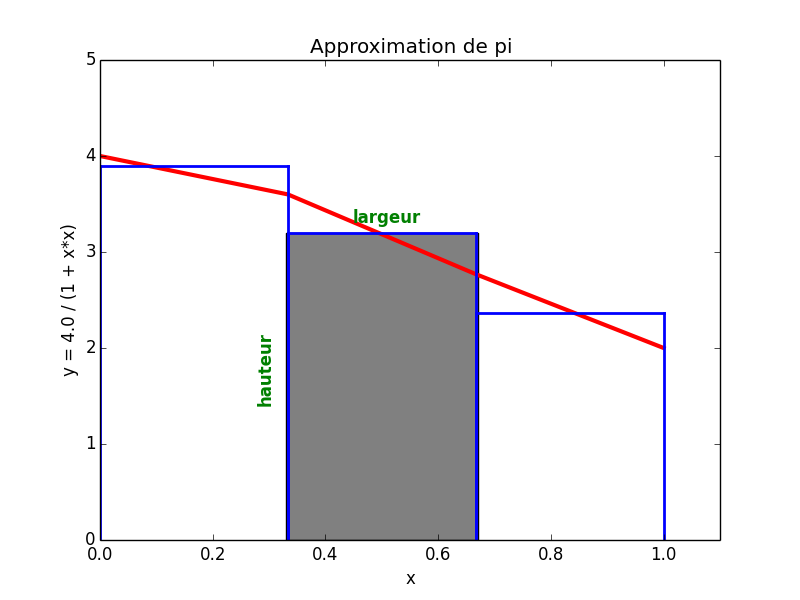
\includegraphics[height=1.8in]{images/Chapitre1/pic_pi_rect_1.png}
        \caption{Approximation avec 4 rectangles}
    \end{subfigure}%
\begin{subfigure}[t]{0.5\textwidth}
        \label{pic_pi_2}
        \centering
        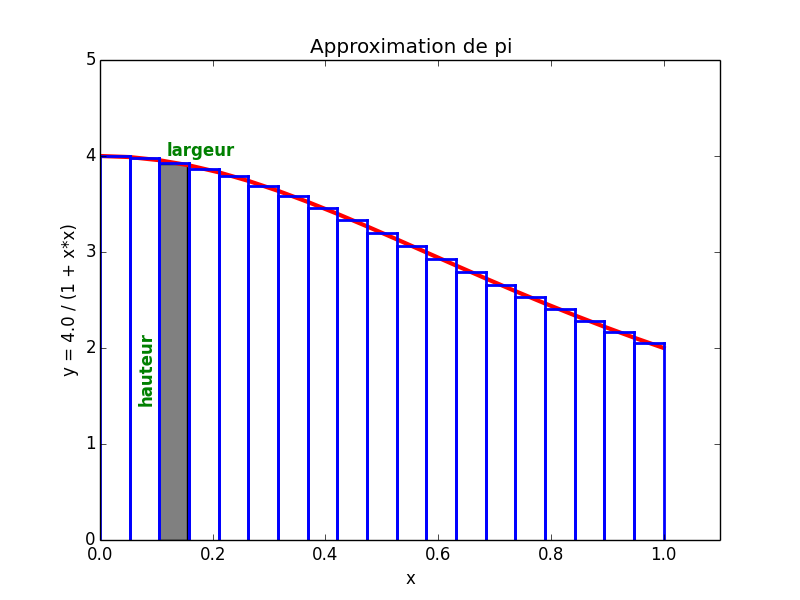
\includegraphics[height=1.8in]{images/Chapitre1/pic_pi_rect_2.png}
        \caption{Approximation avec 14 rectangles}
    \end{subfigure}
    \caption{Méthode des rectangles: exemple de deux exécutions de l'algorithmes un nombre de rectangles différents. Si peu de rectangle sont utilisés cela crée des erreurs. Si on choisit plus de rectangles, on est plus précis, mais plus de ressources sont nécessaires pour le calculer }
    \label{pic_pi_rect}
\end{figure}

\begin{lstlisting}[language=C, caption=Implémentions de l'algorithme de calcul d'intégrale par la méthode des rectangles, float,floatplacement=H]

static long num steps = 100000; 
double step;
void main ()
{
    double largeur, hauteur, pi = 0.0;

    int num_steps = 4;
    //  num_steps = 14;

    largeur = 1.0 / num_steps;

    for (i = 0; i < num_steps; ++i) {
        x =  (i) * step;
        hauteur = ( 4.0/(1.0+x*x));
        pi += largeur * hauteur;
    }
    
    cout << "Valeur de pi: " << pi << endl;

}
\end{lstlisting}



La précision du calcul dépendra du nombre de rectangle choisi, mais approximer l'intégrale avec plus de rectangle demandera plus de ressources informatiques. Si on veut que tous les rectangles soient calculés en même temps il faudra avoir autant de processeurs que de rectangles. C'est un exemple, bien que simpliste, qui montre que la précision des calculs est directement dépendantes du nombre de ressources calculatoire si on veut que le calcul soit résolu dans le même temps. Cet exemple à pour but de montrer que la demande de ressources de calculs est infinis. Dès lors que l'on voudra avoir des résultats plus rapidement, on aura alors besoin d'ordinateurs plus puissants. Et aujourd'hui ces demandes sont réelles, on pourrait évoquer les voitures autonomes qui vont avoir besoin de prendre des décisions en quelques millisecondes. Mais cette logique n'est pas vrai pour un nombre de processeurs infinis et c'est aussi une des motivations de cette thèse. En effet, la loi d'Amdlahl exprime comment la performance est impacté par le nombre de processeurs utilisés.
 



\subsubsection{La loi d'Amdahl} 

\paragraph{La scalabilité TODO}
To get good speedup on a multiprocessor while keeping the problem size fixed is harder than getting good speedup by increasing the size of the problem
Strong scaling:  When speedup is achieved on a parallel processor without increasing the size of the problem
Weak scaling:  When speedup is achieved on a parallel processor by increasing the size of the problem proportionally to the increase in the number of processors

strong
weak

 Il est  souvent impossible de réduire le temps d'exécution du même facteur que le nombre de machines dont on dispose. En effet, les codes comporteront toujours des parties dites séquentiels qui ne peuvent pas être exécutées en parallèle. L'accélération de l'exécution en fonction de la taille de ces parties séquentiels peut être exprimé avec la loi d'Amdahl.

Elle exprime l'accélération du temps d'exécution que l'on peut espérer en fonction des portions de codes qui peuvent être exécuté en parallèle (\autoref{eq_amdahl}). En 1960, Gene Amdahl explique que même si 99\% du code était exécutable en parallèle l'accélération de ce code serait limitée et cela sans regard du nombre de processeurs disponibles. Dans cette équation $P$ représente la portion de code qui peut être exécutée en parallèle et $N$ le nombre de processeurs disponibles.

\begin{equation}
\label{eq_amdahl}
    Speedup (N) = \frac{1}{(1-P) + \frac{P}{N}}
\end{equation}

\begin{figure}
    \center
    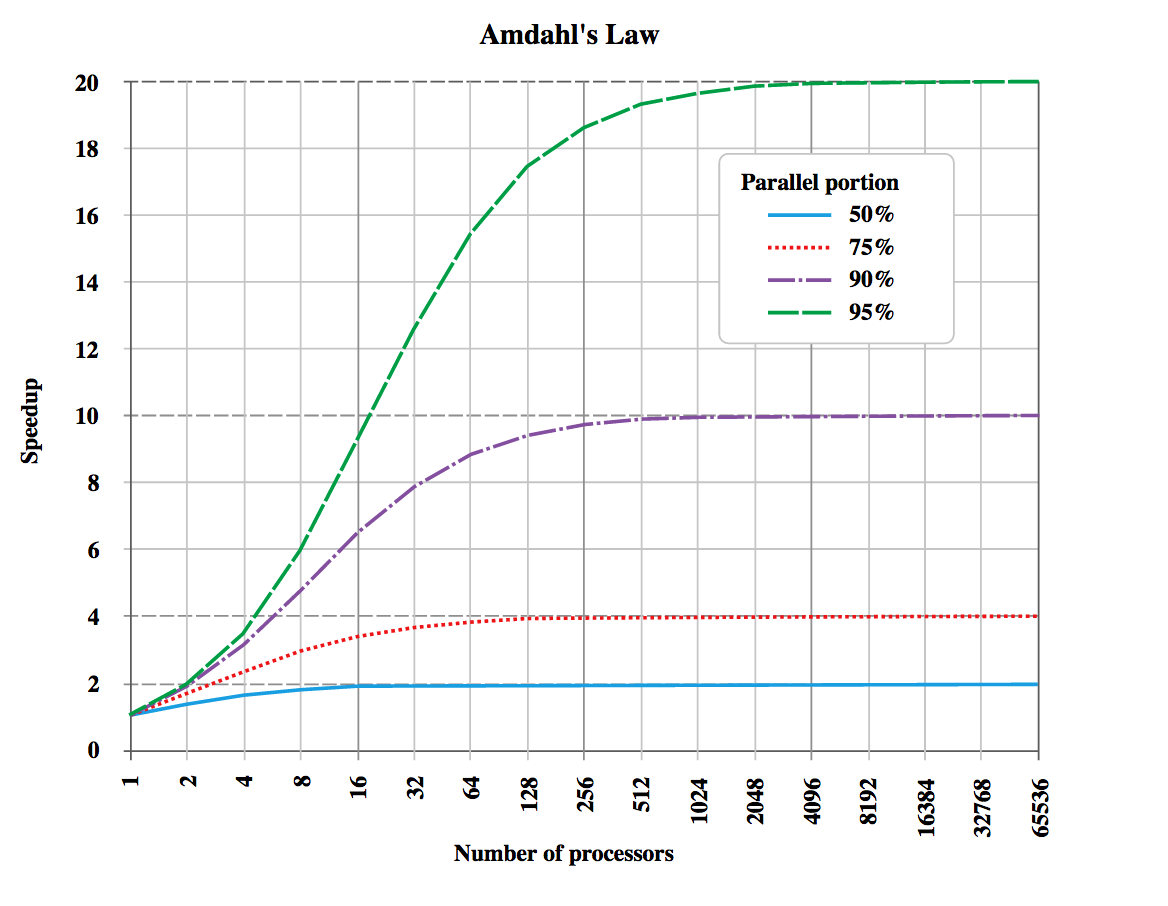
\includegraphics[width=10cm]{images/Chapitre1/AmdahlsLaw.png}
    \caption{\label{pic_amdahl} La loi d'Amdahl décrit l'accélération théorique en fonction du nombre de processeurs pour des codes avec des zones parallèles de différentes taille (source \url{https://fr.wikipedia.org/wiki/Loi\_d\%27Amdahl}).}
\end{figure}

\paragraph{Loi de Gustafson TODO}

TODO faire référence aux different niveaux de parallelisme Taxonomie etc...










%%%%%%%%%%%%%%%%%%%%%%%%%%%%%%%%%%%%%%%%%%%%%%%%%%%%%%%%%%%%%%%
%%%%%%%%%%%%%%%%%%%%%%%%%%%%%%%%%%%%%%%%%%%%%%%%%%%%%%%%%%%%%%%
\subsection{Granularité de parallélisme}

\subsubsection{Parallélisme des instructions (ILP)}
Exemple de deux instructions qui peuvent etre executée séparément
ILP - Instruction
	Superscalar
	Aide: unrolling
	
\subsubsection{Parallélisme des données (DLP)}
- Partition the data used in solving the problem among the cores.
–  Each core carries out similar operations on it s part of the data.

DLP - Data
	SIMD vector
	Aide: blocking, squewing
	Parallel data structures
	
MMX SSE...
One of the issues in parallel program design is the use of Array-Of-Structures (AOS) vs Structure-OfArrays
(SOA). In normal program design you often define a structure
	
Data center
MPI
$https://www.polyhedron.com/web_images/intel/productbriefs/3a_SIMD.pdf$

Exemple d'une multiplication de A * B


\subsubsection{Parallélisme de taches (TLP)}
task parallelism is about identifying whole
subprograms that can be executed in parallel. As an example, searching in a tree data structure
Partition various tasks carried out solving the problem among the
cores.


%%%%%%%%%%%%%%%%%%%%%%%%%%%%%%%%%%%%%%%%%%%%%%%%%%%%%%%%%%%%%%%
%%%%%%%%%%%%%%%%%%%%%%%%%%%%%%%%%%%%%%%%%%%%%%%%%%%%%%%%%%%%%%%
\subsection{La programmation parallèle}
La mémoire est plus grande que le nombre de coeurs. On peut pas avoir un process par data. Il faut donc regrouper, faire des sous tableaux. TODO: exemple de repartition BCN tab [i*myrank].

 


\subsubsection{Parallesisme des threads}

\paragraph{}{Les threads}
Definition des thread: thead vs program.Processes can belong to different users, or be different programs that a single user is running concurrently,
so they have their own data space. On the other hand, threads are part of one process and therefore share
the process heap. Threads can have some private data, for instance

The thread mechanism has long existed, even on a single processor. By having more than one thread on
a single processor, a higher processor utilization can result, since the instructions of one thread can be
processed while another thread is waiting for data

Since threads share data, they are one possible mechanism for parallel programming. Of course, for this to be faster than sequential single-threaded execution, this assumes that the hardware can work on more than one thread at the same time. This can happen in two main circumstances: a multicore processor can accomodate one thread per core, and secondly, some cores have hardware support for executing more than one thread.  processor cores can be an easy way to parallelize a
computation. The shared memory allows the threads to all see the same data.

\paragraph{Exemple OpenMP}
$https://hal.archives-ouvertes.fr/hal-01257189/document p97$



\subsubsection{Data races, thread safety, sequential consistency, and atomic operations }






%%%%%%%%%%%%%%%%%%%%%%%%%%%%%%%%%%%%%%%%%%%%%%%%%%%%%%%%%%%%%%%%%%%%
%%%%%%%%%%%%%%%%%%%%%%%%%%%%%%%%%%%%%%%%%%%%%%%%%%%%%%%%%%%%%%%%%%%%
%%%%%%%%%%%%%%%%%%%%%%%%%%%%%%%%%%%%%%%%%%%%%%%%%%%%%%%%%%%%%%%%%%%%
%%%%%%%%%%%%%%%%%%%%%%%%%%%%%%%%%%%%%%%%%%%%%%%%%%%%%%%%%%%%%%%%%%%%
%%%%%%%%%%%%%%%%%%%%%%%%%%%%%%%%%%%%%%%%%%%%%%%%%%%%%%%%%%%%%%%%%%%%
%%%%%%%%%%%%%%%%%%%%%%%%%%%%%%%%%%%%%%%%%%%%%%%%%%%%%%%%%%%%%%%%%%%%
%%%%%%%%%%%%%%%%%%%%%%%%%%%%%%%%%%%%%%%%%%%%%%%%%%%%%%%%%%%%%%%%%%%%
%%%%%%%%%%%%%%%%%%%%%%%%%%%%%%%%%%%%%%%%%%%%%%%%%%%%%%%%%%%%%%%%%%%%
%%%%%%%%%%%%%%%%%%%%%%%%%%%%%%%%%%%%%%%%%%%%%%%%%%%%%%%%%%%%%%%%%%%%
%%%%%%%%%%%%%%%%%%%%%%%%%%%%%%%%%%%%%%%%%%%%%%%%%%%%%%%%%%%%%%%%%%%%
%%%%%%%%%%%%%%%%%%%%%%%%%%%%%%%%%%%%%%%%%%%%%%%%%%%%%%%%%%%%%%%%%%%%
%%%%%%%%%%%%%%%%%%%%%%%%%%%%%%%%%%%%%%%%%%%%%%%%%%%%%%%%%%%%%%%%%%%%
%%%%%%%%%%%%%%%%%%%%%%%%%%%%%%%%%%%%%%%%%%%%%%%%%%%%%%%%%%%%%%%%%%%%
%%%%%%%%%%%%%%%%%%%%%%%%%%%%%%%%%%%%%%%%%%%%%%%%%%%%%%%%%%%%%%%%%%%%
%%%%%%%%%%%%%%%%%%%%%%%%%%%%%%%%%%%%%%%%%%%%%%%%%%%%%%%%%%%%%%%%%%%%
%%%%%%%%%%%%%%%%%%%%%%%%%%%%%%%%%%%%%%%%%%%%%%%%%%%%%%%%%%%%%%%%%%%%
%%%%%%%%%%%%%%%%%%%%%%%%%%%%%%%%%%%%%%%%%%%%%%%%%%%%%%%%%%%%%%%%%%%%
%%%%%%%%%%%%%%%%%%%%%%%%%%%%%%%%%%%%%%%%%%%%%%%%%%%%%%%%%%%%%%%%%%%%



\section{Sommaire}

Alors que nous n'avons jamais eu besoin d'aussi grandes puissances de calcul, le graphique montre bien qu'il y a eu une inflexion en 2012. Le challenge principal inhérent au HPC est celui du cout des machines et donc celui du ratio $\frac{Prix}{FLOPS}$. Un autre challenge qui est apparu est celui de la puissance électrique nécessaire pour aliment les supercalculateurs. Les lignes électrique arrivant sur les sites, ne sont plus assez puissante pour que l'on puisse suivre la stratégie employée jusqu'à aujourd'hui qui était d'augmenter le nombre de machines pour augmenter la puissance de calcul. Aujourd'hui nous cherchons donc aussi à augmenter le ratio $\frac{Watt}{FLOPS}$ même si cette solution ne sera pas éternellement viable comme l'a prédit \cite{5392446}.
Enfin, les clients du HPC acquièrent plus de données que jamais et les clusters doivent pouvoir les contenir et les traiter dans des délais raisonnable. En effet les objets connectés qui génèrent de gigantesques quantité de données doivent être capables d'en traiter une partie sur place avec des moyens souvent limité (énergie, puissance de calculs). Ces challenges sont donc applicables au data center mais aussi à l'extérieur si nous voulons être capable de prendre des décisions en temps réel, comme pour les voitures autonomes qui n'auront que quelques micro secondes pour réagir en cas d'accident. Le travail présenté dans cette thèse est donc nécessaire pour pouvoir accéder à toutes ces promesses que nous réserve l'avenir.


\subsubsection{Systèmes non-équilibrés}

La précision des simulations, les approches multi-physique ainsi que les objets connectés produisent des volumes de données à gérer et à analyser tels qu’ils ont été caractérisé par la communauté de déluge %\cite{bodin:hal-01174302}.
En conséquence, l’exploitation et la gestion des données sont l’autre pan de l’évolution des logicielles qui va bouleverser les pratiques. Une majorité des applications HPC autrefois centrée sur une problématique de puissance de calcul sont maintenant fortement limitées par le traitement des données pour deux raisons: une augmentation très forte de la puissance des processeurs contre une faible augmentation de la quantité de données que les mémoires peuvent leur délivrer. Si on regarde l'évolution des performances des différentes parties du système on peut constater de réelles différences:
\begin{itemize}
    \item Les performances calculatoirs des processeurs (le nombre d'opération flotantes réalisables par cycle) à \textbf{augmenté de 50\%} en moyenne par an.
    \item La bande passante entre le processeur et la mémoire à augmenté de 23\% par an
    \item La lantence des requêtes mémoire a \textbf{augmenté de 4\% }par an
    \item La bande passante sur le réseau à \textbf{augmenté de 20\%} par an
\end{itemize}

\begin{figure}
    \center
    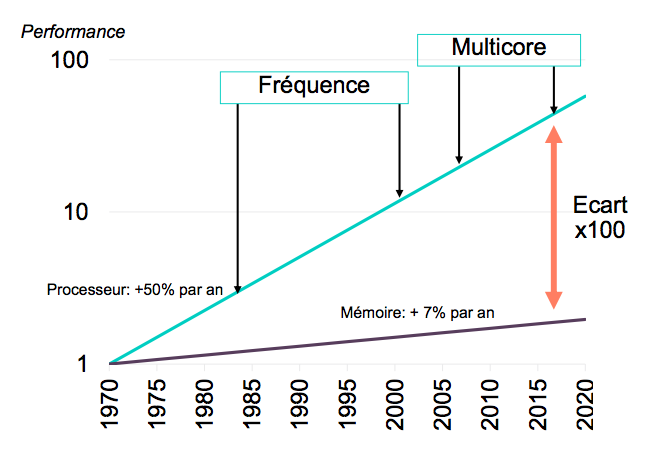
\includegraphics[width=10cm]{images/Chapitre1/memory_gap.png}
    \caption{\label{pic_memory_gap} Différence de l'évolution des performances des processeurs et des mémoires }
\end{figure}

On voit donc que la puissance des processeurs à augmenté bien plus rapidement que celle des mémoires. Les processeurs ont béféniciés de nombreuse amélioration. L'augmentation de la fréquences par exemple, ou le nombre de coeurs par processeur. Ainsi les performances des systèmes ne sont plus équilibrées et les architectures ont du s'adapter notamment avec l'apparition d'une hierarchie mémoire, plus au moins rapide et plus ou moins grande. L'apparition des caches à permis d'augmenter la performance relative des applications en camouflant l'augmentation faible de la bande passante. Cela à contribué à l'augmentation de la complexité des architectures et il faut désormais au programmeur des connaissances solides pour aller tirer le maximum de performances de ces processeurs

\textbf{TODO: annoncer le plan de these}



%%%%%%%%%%%%%%%%%%%%%%%%%%%%%%%%%%%%%%%%%%%%%%%%%%%%%%%%%%%%%%%%%%%%
%%%%%%%%%%%%%%%%%%%%%%%%%%%%%%%%%%%%%%%%%%%%%%%%%%%%%%%%%%%%%%%%%%%%
%%%%%%%%%%%%%%%%%%%%%%%%%%%%%%%%%%%%%%%%%%%%%%%%%%%%%%%%%%%%%%%%%%%%
%%%%%%%%%%%%%%%%%%%%%%%%%%%%%%%%%%%%%%%%%%%%%%%%%%%%%%%%%%%%%%%%%%%%
%%%%%%%%%%%%%%%%%%%%%%%%%%%%%%%%%%%%%%%%%%%%%%%%%%%%%%%%%%%%%%%%%%%%
%%%%%%%%%%%%%%%%%%%%%%%%%%%%%%%%%%%%%%%%%%%%%%%%%%%%%%%%%%%%%%%%%%%%
%%%%%%%%%%%%%%%%%%%%%%%%%%%%%%%%%%%%%%%%%%%%%%%%%%%%%%%%%%%%%%%%%%%%
%%%%%%%%%%%%%%%%%%%%%%%%%%%%%%%%%%%%%%%%%%%%%%%%%%%%%%%%%%%%%%%%%%%%
%%%%%%%%%%%%%%%%%%%%%%%%%%%%%%%%%%%%%%%%%%%%%%%%%%%%%%%%%%%%%%%%%%%%
%%%%%%%%%%%%%%%%%%%%%%%%%%%%%%%%%%%%%%%%%%%%%%%%%%%%%%%%%%%%%%%%%%%%
%%%%%%%%%%%%%%%%%%%%%%%%%%%%%%%%%%%%%%%%%%%%%%%%%%%%%%%%%%%%%%%%%%%%
%%%%%%%%%%%%%%%%%%%%%%%%%%%%%%%%%%%%%%%%%%%%%%%%%%%%%%%%%%%%%%%%%%%%
%%%%%%%%%%%%%%%%%%%%%%%%%%%%%%%%%%%%%%%%%%%%%%%%%%%%%%%%%%%%%%%%%%%%
%%%%%%%%%%%%%%%%%%%%%%%%%%%%%%%%%%%%%%%%%%%%%%%%%%%%%%%%%%%%%%%%%%%%
%%%%%%%%%%%%%%%%%%%%%%%%%%%%%%%%%%%%%%%%%%%%%%%%%%%%%%%%%%%%%%%%%%%%
%%%%%%%%%%%%%%%%%%%%%%%%%%%%%%%%%%%%%%%%%%%%%%%%%%%%%%%%%%%%%%%%%%%%
%%%%%%%%%%%%%%%%%%%%%%%%%%%%%%%%%%%%%%%%%%%%%%%%%%%%%%%%%%%%%%%%%%%%
%%%%%%%%%%%%%%%%%%%%%%%%%%%%%%%%%%%%%%%%%%%%%%%%%%%%%%%%%%%%%%%%%%%%




TODO 
\label{sub_taxonomie}
%\cite{Flynn:1972:COE:1952456.1952459}
$https://www.polyhedron.com/web_images/intel/productbriefs/3a_SIMD.pdf$
schéma nombre d'opération par cycle et aussi que 4xfloat = 2 double = 16xbytes ...

\printbibliography[heading=references,segment=\therefsegment]
